% Opsætter KU Tex dokument
%%%%%%%%%%%%%%%%%%%%%%%%%%%%%%%%%%%%%%%%%%%%%%%%%%%%%%%%%%%%%%%%%%%%%%%%%%%%%%%%
\documentclass{article}                                                        %
\usepackage[a4paper, hmargin={2.8cm, 2.8cm}, vmargin={2.5cm, 2.5cm}]{geometry} %
\usepackage{eso-pic}  % \AddToShipoutPicture                                   %
\usepackage{graphicx} % \includegraphics                                       %
%\usepackage{subfig} - Can not be used with subcaption package (for subfigures)
\usepackage{setspace}                                                        %
%%%%%%%%%%%%%%%%%%%%%%%%%%%%%%%%%%%%%%%%%%%%%%%%%%%%%%%%%%%%%%%%%%%%%%%%%%%%%%%%

% Pakker til skrifttyper, tekst osv.
%%%%%%%%%%%%%%%%%%%%%%%%%%%%%%%%%%%%%%%%%%%%%%%%%%%%%%%%%%%%%%%%%%%%%%%%%%%%%%%%
    \usepackage[utf8]{inputenc}  % Implementere Unicode                        %
    \usepackage[T1]{fontenc}     % Unicode skrifttype fx. é skrives som 1 tegn %
    \usepackage[english]{babel}   % Dansk Ordbog                                %
    \usepackage{microtype}       % Forbedre linjeombrydningen                  %
    \usepackage{libertine}       % Skrifttype                                  %
%%%%%%%%%%%%%%%%%%%%%%%%%%%%%%%%%%%%%%%%%%%%%%%%%%%%%%%%%%%%%%%%%%%%%%%%%%%%%%%%

% Pakker til matematik og kode.
%%%%%%%%%%%%%%%%%%%%%%%%%%%%%%%%%%%%%%%%%%%%%%%%%%%%%%%%%%%%%%%%%%%%%%%%%%%%%%%%
    \usepackage{mathtools}       % Udvidelse til amsmath pakken                %
    \usepackage{amsthm}          % Pakke til bevisførelse                      %
    \usepackage{amssymb}         % Extra matematiske symboler                  %				
	%\usepackage{mychemistry}												   %
%	%\usepackage[version=3]{mhchem}											   %
	\usepackage{wrapfig}													   %
	\usepackage{siunitx}	
	\usepackage{anyfontsize}
	\usepackage{ragged2e}
	\usepackage{algorithm2e}
	\usepackage[final]{pdfpages}
	\usepackage{listings}
	\usepackage{tikz}
	\usepackage{multirow}
	\usepackage{makecell}
	\usepackage{fourier} 
	\usepackage{array}
	\usepackage{todonotes}
	\usepackage{pdflscape}
	\usetikzlibrary{arrows,shapes}
	\usepackage{titlesec}
	\usepackage{hyperref}
	\usepackage{url}
	\usepackage[nottoc,numbib]{tocbibind}
	\usepackage{semantic}
	\usepackage{subcaption}
	\usepackage{qtree}
	\usepackage{hhline}
	
	\definecolor{light-gray}{gray}{0.85}
	\lstset{
	    	numbers=left,
	    	breaklines=true,
	    	backgroundcolor=\color{light-gray},
	    	tabsize=2,
	    	basicstyle=\ttfamily,
	    	literate={\ \ }{{\ }}1
	}
	
	\urlstyle{same}
	\tikzstyle{vertex}=[circle,fill=white!25,minimum size=20pt,inner sep=0pt]
	\tikzstyle{edge} = [draw,thick,-]

	\definecolor{light-gray}{gray}{0.85}
	\definecolor{dkgreen}{RGB}{0.0,128.0,43.0}
	\lstdefinelanguage{FSharp}%
{morekeywords={new, match, with, rec, open, module, namespace, type, of, member, % 
and, for, while, true, false, in, do, begin, fun, function, return, yield, try, %end
mutable, if, then, else, cloud, async, static, use, abstract, interface, inherit, finally, int },
  otherkeywords={ let!, return!, do!, yield!, use!, var, from, select, where, order, by },
  keywordstyle=\color{bluekeywords},
  sensitive=true,
  basicstyle=\ttfamily,
	breaklines=true,
  xleftmargin=\parindent,
  aboveskip=\bigskipamount,
	tabsize=4,
  morecomment=[l][\color{dkgreen}]{///},
  morecomment=[l][\color{dkgreen}]{//},
  morecomment=[l][\color{dkgreen}]{(*},
  morecomment=[s][\color{dkgreen}]{},
  morestring=[b]",
  showstringspaces=false,
  literate={`}{\`}1,
  stringstyle=\color{redstrings},
}
	
	
												   %
%%%%%%%%%%%%%%%%%%%%%%%%%%%%%%%%%%%%%%%%%%%%%%%%%%%%%%%%%%%%%%%%%%%%%%%%%%%%%%%%

% Pakker til layout.
%%%%%%%%%%%%%%%%%%%%%%%%%%%%%%%%%%%%%%%%%%%%%%%%%%%%%%%%%%%%%%%%%%%%%%%%%%%%%%%%
    \usepackage{fancyhdr}            % Gør det muligt at bruge sidehoveder     %
    \usepackage{graphicx}            % Mulighed for bl.a. \includegraphics     %
    \usepackage{colortbl}            % Hvis man vil farvelægge sine tabeller   %
    \usepackage{array}               % Gør miljøerne array og tabular bedre    %
    \usepackage{parskip}             % Første paragraf i afsnit indrykkes ikke %
    \usepackage{titlesec}            % Tilpassing af afstand mellem sektioner  %
    \usepackage[lastpage,user]{zref} % Side x af y                             %
%%%%%%%%%%%%%%%%%%%%%%%%%%%%%%%%%%%%%%%%%%%%%%%%%%%%%%%%%%%%%%%%%%%%%%%%%%%%%%%%


% Implementerer en række makroer og de pakker der er importeret
%%%%%%%%%%%%%%%%%%%%%%%%%%%%%%%%%%%%%%%%%%%%%%%%%%%%%%%%%%%%%%%%%%%%%%%%%%%%%%%%
    \pagestyle{fancy}                        % Implementerer sidehoved         %
    \lhead{University of Copenhagen}                % Venstre sidehoved               %
    \rhead{Exam number: 13}                             % Højre sidehoved      %
    \cfoot{\thepage\ of \zpageref{LastPage}} % Side x af y                     %
    \newtheorem*{prp}{Propostion}            % Skaber nyt theorem  
    \renewcommand{\baselinestretch}{1.25}       %
%%%%%%%%%%%%%%%%%%%%%%%%%%%%%%%%%%%%%%%%%%%%%%%%%%%%%%%%%%%%%%%%%%%%%%%%%%%%%%%%

% Mindsker afstanden mellem sektioner
%%%%%%%%%%%%%%%%%%%%%%%%%%%%%%%%%%%%%%%%%%%%%%%%%%%%%%%%%%%%%%%%%%%%%%%%%%%%%%%%%%
\titlespacing\section{0pt}{12pt plus 4pt minus 2pt}{0pt plus 1pt minus 3pt}      %
\titlespacing\subsection{0pt}{12pt plus 4pt minus 2pt}{0pt plus 1pt minus 3pt}   %
\titlespacing\subsubsection{0pt}{12pt plus 4pt minus 2pt}{0pt plus 1pt minus 3pt}%
%%%%%%%%%%%%%%%%%%%%%%%%%%%%%%%%%%%%%%%%%%%%%%%%%%%%%%%%%%%%%%%%%%%%%%%%%%%%%%%%%%

%Ændrer størelsen på sections
%%%%%%%%%%%%%%%%%%%%%%%%%%%%%%%%%%%%%%%%%%%%%%%%%%%%%%%%%%%%%%%%%%%%%%%%%%%%%%%%%%
\titleformat{\section}
{\normalfont\fontsize{14}{16}\bfseries}{\thesection}{1em}{}
\titleformat{\subsection}
{\normalfont\fontsize{12}{14}\bfseries}{\thesubsection}{1em}{}
\titleformat{\subsubsection}
{\normalfont\fontsize{11}{13}\bfseries}{\thesubsubsection}{1em}{}
%%%%%%%%%%%%%%%%%%%%%%%%%%%%%%%%%%%%%%%%%%%%%%%%%%%%%%%%%%%%%%%%%%%%%%%%%%%%%%%%%%

%%%%%%%%%%%%
% Document %
%%%%%%%%%%%%

\begin{document}

\begin{titlepage}

\newcommand{\HRule}{\rule{\linewidth}{0.5mm}} % Defines a new command for the horizontal lines, change thickness here

\begin{center}
 % Center everything on the page
 
%----------------------------------------------------------------------------------------
%	HEADING SECTIONS
%----------------------------------------------------------------------------------------

\textsc{\LARGE University of Copenhagen}\\[1.5cm] % Name of your university/college
\textsc{\Large Computer Science}\\[0.5cm] % Major heading such as course name
\textsc{\large Advanced Topics in Image Analysis}\\[0.5cm] % Minor heading such as course title

%----------------------------------------------------------------------------------------
%	TITLE SECTION
%----------------------------------------------------------------------------------------

\HRule \\[0.4cm]
{ \huge \bfseries Exam project}\\[0.4cm] % Title of your document
\HRule \\[1.5cm]
 
%----------------------------------------------------------------------------------------
%	AUTHOR SECTION
%----------------------------------------------------------------------------------------

\begin{minipage}{0.4\textwidth}
\begin{flushleft} \large
\emph{Author:}\\ 
% Your name
Exam number: 13 \\
\hfill
\end{flushleft}
\end{minipage}
~
\begin{minipage}{0.4\textwidth}
\begin{flushright} \large
\emph{Teachers:} \\
Søren \textsc{Olsen}\\
Sune  \textsc{Darkner}
\end{flushright}
\end{minipage}\\[2cm]

% If you don't want a supervisor, uncomment the two lines below and remove the section above
%\Large \emph{Forfattere:}\\
%Axel \textsc{Christof}\\% Your name
%Casper \textsc{Bresdahl}\\
%Emilie \textsc{Bentsen}\\[1cm] 

%----------------------------------------------------------------------------------------
%	DATE SECTION
%----------------------------------------------------------------------------------------

{\large \today}\\[2cm] % Date, change the \today to a set date if you want to be precise

%----------------------------------------------------------------------------------------
%	LOGO SECTION
%----------------------------------------------------------------------------------------


\includegraphics{logo.png}\\[1cm] % Include a department/university logo - this will require the graphicx package
 
%----------------------------------------------------------------------------------------

\vfill % Fill the rest of the page with whitespace

%Disse linjer skaber forside, evt indholdsfortegnelse, og sætter sidetal
%%%%%%%%%%%%%%%%%%%%%%%%%%%%%%%%%%%%%%%%%%%%%%%%%%%%%%%%%%%%%%%%%%%%%%%%%%%%%%%%
									                                           %
    \thispagestyle{empty}   % Fjerner sidetal forside                          %
        % Slå disse til hvis der ønskes indholdsfortegnelse                    %
        %%%%%%%%%%%%%%%%%%%%%%%%%%%%%%%%%%%%%%%%%%%%%%%%%%%%%%%%%%%%%%%%%%%%%%%% 
            \newpage                % Side til indholdsfortegnelse            %
            %\thispagestyle{empty}   % Fjerner sidetal fra indholdsfortegnelse %
            %\tableofcontents        % Skaber indholdsfortegnelse              %
    \end{center}
    %\section*{Forord}
    	
		
        %%%%%%%%%%%%%%%%%%%%%%%%%%%%%%%%%%%%%%%%%%%%%%%%%%%%%%%%%%%%%%%%%%%%%%%%
    \newpage                % Første rigtige side
    \setcounter{page}{1}    % Sætter rigtigt sidetal på første side
%%%%%%%%%%%%%%%%%%%%%%%%%%%%%%%%%%%%%%%%%%%%%%%%%%%%%%%%%%%%%%%%%%%%%%%%%%%%%

\end{titlepage}
{\fontsize{10}{14}\selectfont
\section{Assignment 1}
\subsection{Baseline}
\begin{figure}[h]
	\centering
	\begin{subfigure}{0.48\linewidth}
		\centering
		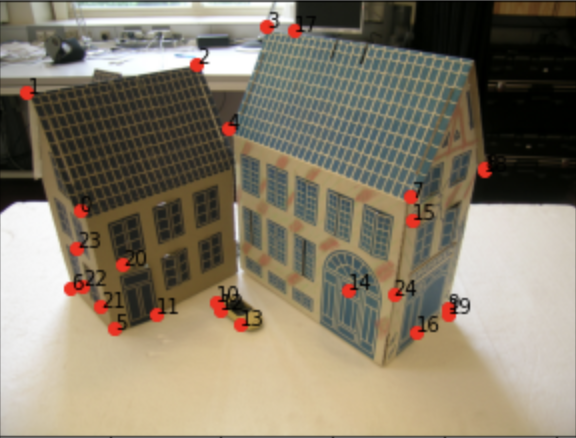
\includegraphics[width=\linewidth]{Materials/BaselineA}
	\end{subfigure}
	\hfill
	\begin{subfigure}{0.48\linewidth}
		\centering
		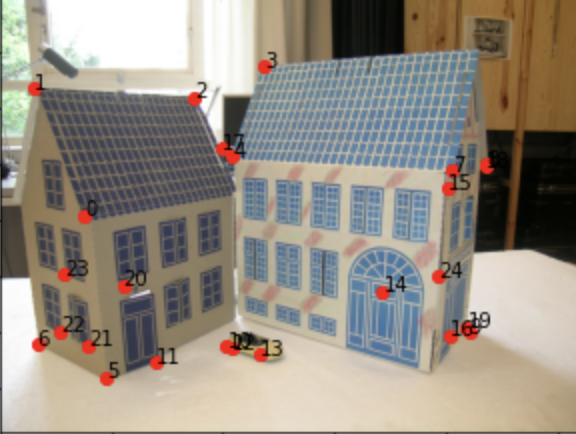
\includegraphics[width=\linewidth]{Materials/BaselineB}
	\end{subfigure}
	\caption{The 25 point correspondences between the two images found.}
	\label{correspondences}
\end{figure}
We will begin by establishing a baseline for comparison with the following experiments. This baseline will be the most naive / simple solution to estimating the fundamental matrix and bring the two images to scanline agreement. We begin by manually estimating 25 point correspondences between the two images which can be seen in \autoref{correspondences}. We now normalize the points found in each image separately by subtracting the mean of the points and dividing with their standard deviation. This gives us $T_A$ and $T_B$ which are transformation matrices for image A (left) and image B (right), and we will use these to denormalize the fundamental matrix. We can now estimate the fundamental matrix using the 8-point algorithm and after normalizing it by dividing through with index (3,3), we can report it to be:
\begin{equation*}
	F = \begin{bmatrix}
		-2.35e-06 & -1.81e-06 & -1.50e-02\\
		2.77e-06 & 2.43e-06 & -2.05e-02\\
		1.99e-02 &1.63e-02 & 1
	\end{bmatrix}
\end{equation*}
With the fundamental matrix we can now use \textit{opencv} and the function \textit{computeCorrespondEpilines} to determine the epipolar lines and draw them on the images by supplying the function with the points found in the images and the estimated fundamental matrix. This is done in \autoref{baselineepipolarlines}. Using opencv is simply for convenience to transform the points and estimating and drawing the epipolar lines.

\begin{figure}[h]
	\centering
	\begin{subfigure}{0.48\linewidth}
		\centering
		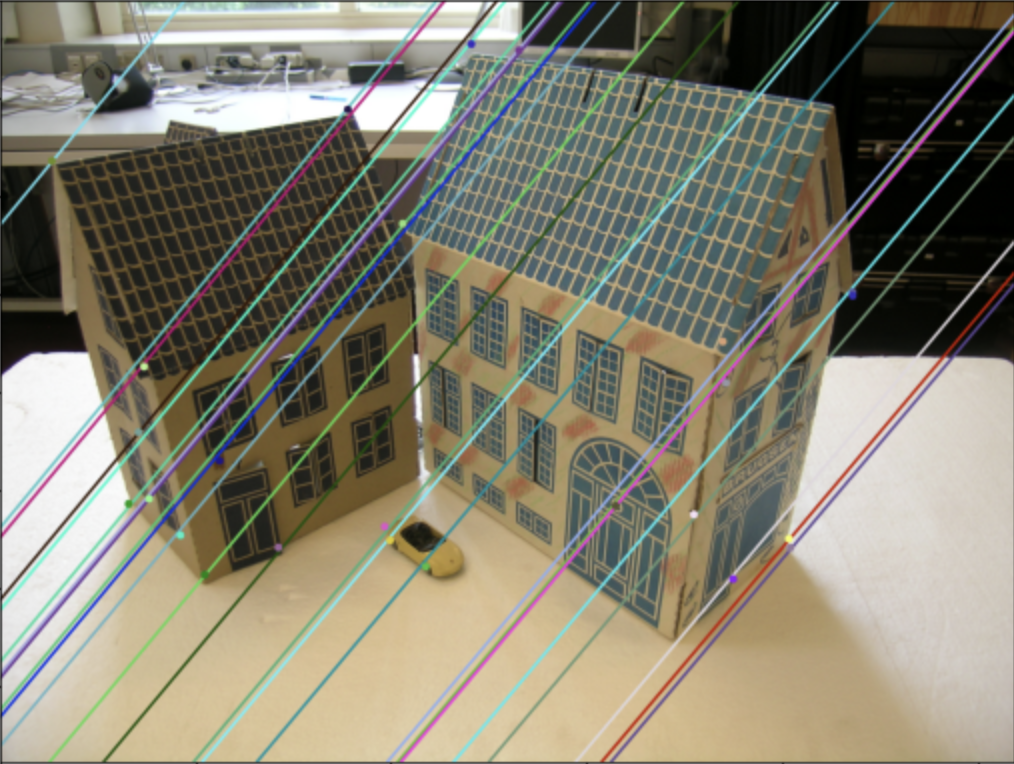
\includegraphics[width=\linewidth]{Materials/BaselineEpiA}
	\end{subfigure}
	\hfill
	\begin{subfigure}{0.48\linewidth}
		\centering
		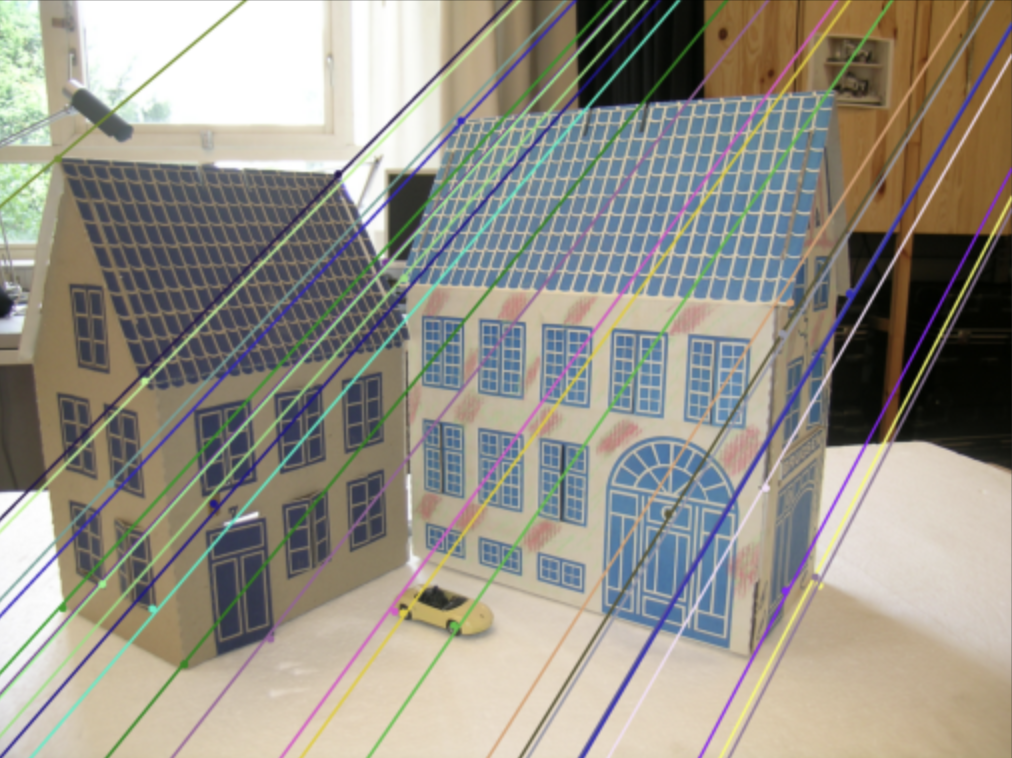
\includegraphics[width=\linewidth]{Materials/BaselineEpiB}
	\end{subfigure}
	\caption{Epipolar lines drawn on top of the two images.}
	\label{baselineepipolarlines}
\end{figure}
By computing the left and right null vectors of the fundamental matrix, $F$, we can get the coordinates of the epipoles. We find the left epipole, i.e. the optical center of the right camera projected into the left cameras view, to be at coordinates $[-104610.58, 127733.71]$, and the right epipole, i.e. the optical center of the left camera projected into the right cameras view, to be $[4577.86, -3312.85]$.\\
We can now bring the two images to scanline agreement using \textit{opencv} which can be seen in \autoref{baselineScanline}.
\begin{figure}[h]
	\centering
	\begin{subfigure}{0.48\linewidth}
		\centering
		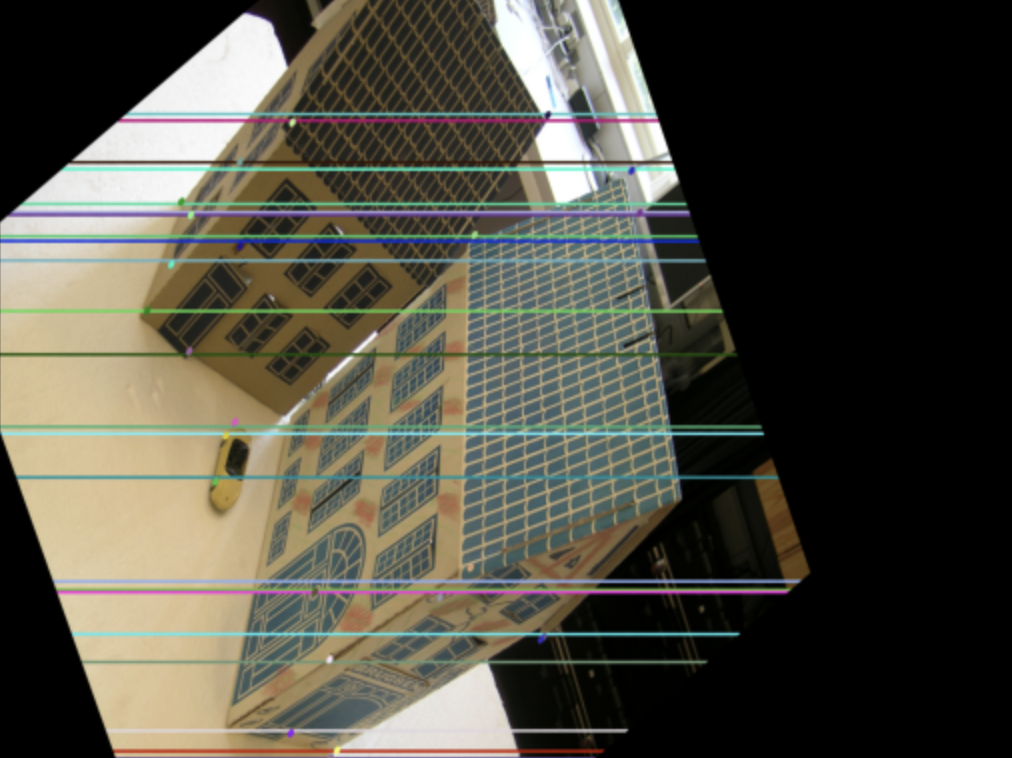
\includegraphics[width=\linewidth]{Materials/BaselineScanlineA}
	\end{subfigure}
	%\hfill
	\begin{subfigure}{0.48\linewidth}
		\centering
		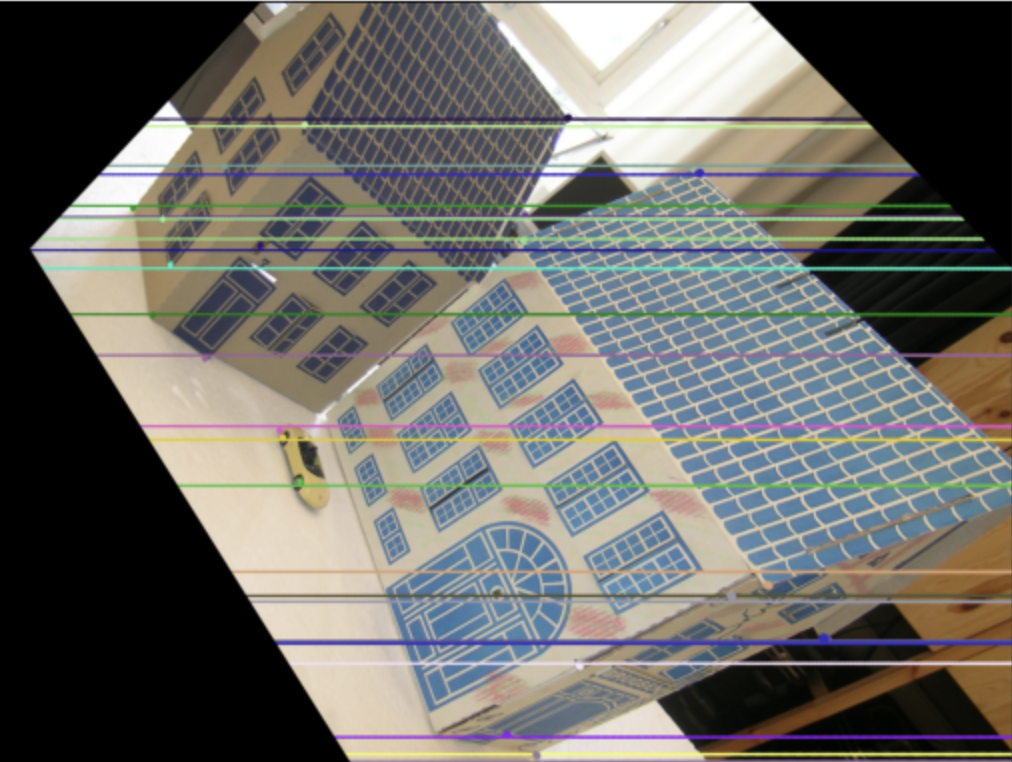
\includegraphics[width=\linewidth]{Materials/BaselineScanlineB}
	\end{subfigure}
	\caption{The baseline estimation brought to scanline agreement.}
	\label{baselineScanline}
\end{figure}
As the 'scanline agreement error' is ambiguous to me, I have chosen to follow the 'rectification error' from \cite{rectificationError} which measures the error by computing the mean and standard deviation of the \textit{y-disparity} (the vertical distance) between the points in image A and image B after rectification. Here we find a \textbf{mean} of \textbf{8.53} and a \textbf{standard deviation} of \textbf{7.41} which tells us our epipolar lines on average are fairly close to go through our points in the images, but the variance is also fairly high, which implies some of our points are very close, and some are quite far off.
\subsection{Ransac with baseline}
Ransac is a procedure which can be used to detect outlying data. We will use Ransac to sort out the correspondences we have found which are too imprecise to contribute to the estimation of the fundamental matrix. Using Ransac makes our estimation of the fundamental matrix more robust, and so we will also look at how robust our estimation becomes by adding random correspondences and then attempt to remove false correspondences with Ransac.

\subsubsection{Problems with Ransac}
Ransac can be implemented in a few different ways. One could simply use the largest inlier set found and return this. One could also estimate the error, and although a bigger inlier set might be found, it will only be accepted if the error is smaller than the previous best set (the set with the smallest error and largest number of inliers). Then, should the points used to compute the model be included when computing this error, or only points not used in the model estimation? In the latter we avoid bias, but the points used for model estimation will most likely be quantified as inliers. And perhaps most importantly, how does one estimate the thresholding used to determine inliers from outliers?\\
After some experimentation I have found using the largest inlier set gave the most consistent results and have thus chosen to use this implementation. For thresholding a constant threshold of 20 have been used. As the threshold is often simply chosen empirically, and the scanline agreement error from the baseline shows decent results, a threshold of 20 seems reasonable. The threshold could also have been estimated based on the standard deviation and a Chi distribution. To determine whether a correspondence is within this threshold, the \textit{Sampson distance} have been used as this seems to the most natural way to estimate the error, and it only involves the fundamental matrix.

\subsubsection{Error as function of falsely added correspondences}
We will now take a look at how robust the fundamental matrix estimation is when using Ransac. For this we take our 25 manually found correspondences and add a number of false correspondence before running Ransac. We then measure the mean and standard deviation of the scanline agreement error. As Ransac is a non-deterministic algorithm we might get rather different errors each run, and because we only are interested in the tendency of how the error behaves when adding false correspondences, we make 10 runs of Ransac and report the median mean and standard deviation found. This helps us avoid lucky or unlucky runs where the error reported is 'uncharacteristic' for the number of false correspondences added, and to avoid the skewness the average would give if one run reports something completely different than the other runs. The results can be seen in \autoref{BaselineRansacMedian}.

\begin{figure}[h]
	\centering
	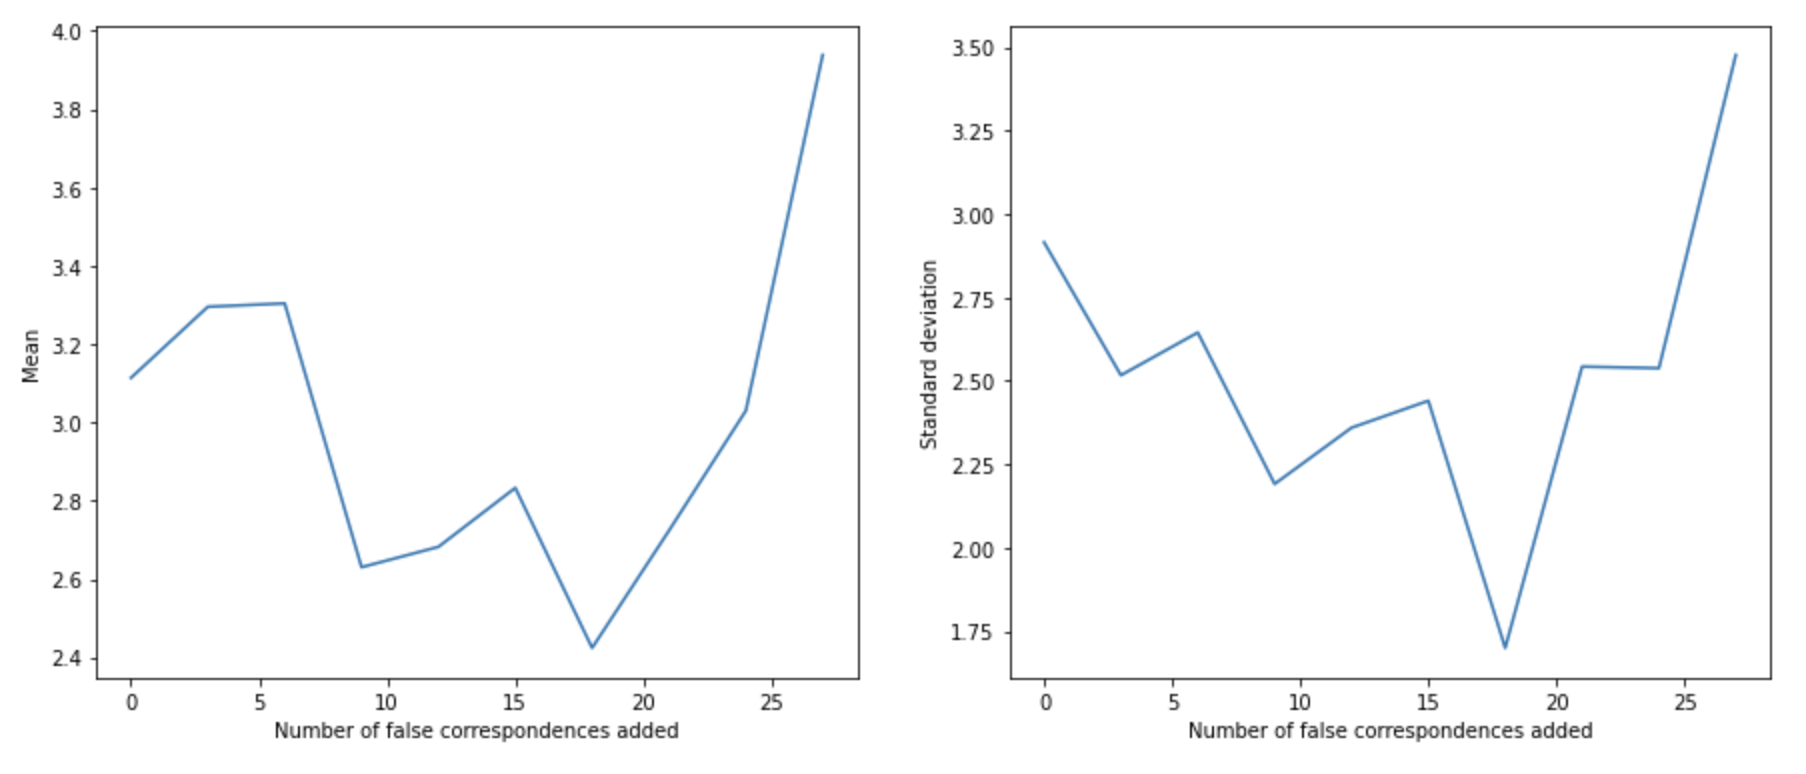
\includegraphics[width=\linewidth]{Materials/BaselineRansacMedian}
	\caption{The median mean and standard deviation after 10 Ransac runs with increasing number of false correspondences added to the manually found correspondences.}
	\label{BaselineRansacMedian}
\end{figure}
As seen the median mean and standard deviation only changes slightly, however, both show a tendency to grow quite rapidly when adding more than 18 false correspondences. This would equate to when the data consists of more than 42\% outliers Ransac begins to break down. This shows using Ransac makes the estimation of the fundamental matrix \textit{very} robust. We do however need to keep in mind that the false correspondences added here are random points in the two images, and so they with high probability fall \textit{completely} out of line with our inliers. This might be a reason why we can include so many false correspondences.

\subsubsection{Scanline agreement using Ransac}
Taking a visual look at using Ransac, we can report the result of running Ransac on the 25 correspondences manually found, and from the inliers, estimate the fundamental matrix. This can be seen in \autoref{BaselineRansac}.
\begin{figure}[h]
	\centering
	\begin{subfigure}{0.48\linewidth}
		\centering
		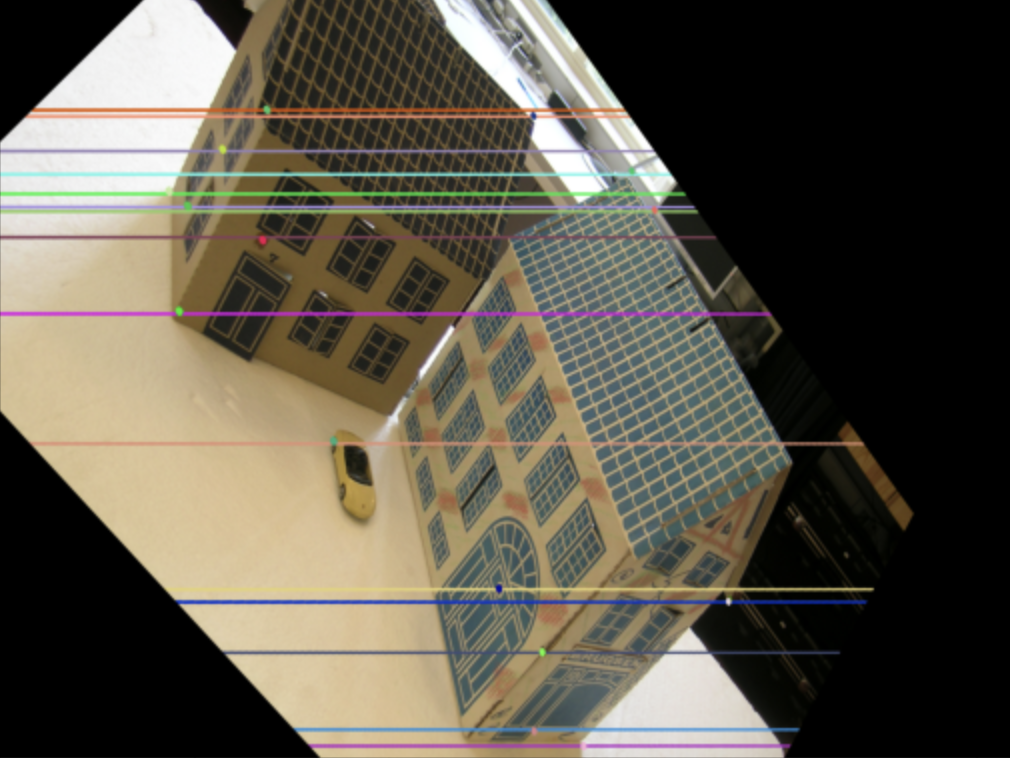
\includegraphics[width=\linewidth]{Materials/BaselineARansac}
	\end{subfigure}
	\begin{subfigure}{0.48\linewidth}
		\centering
		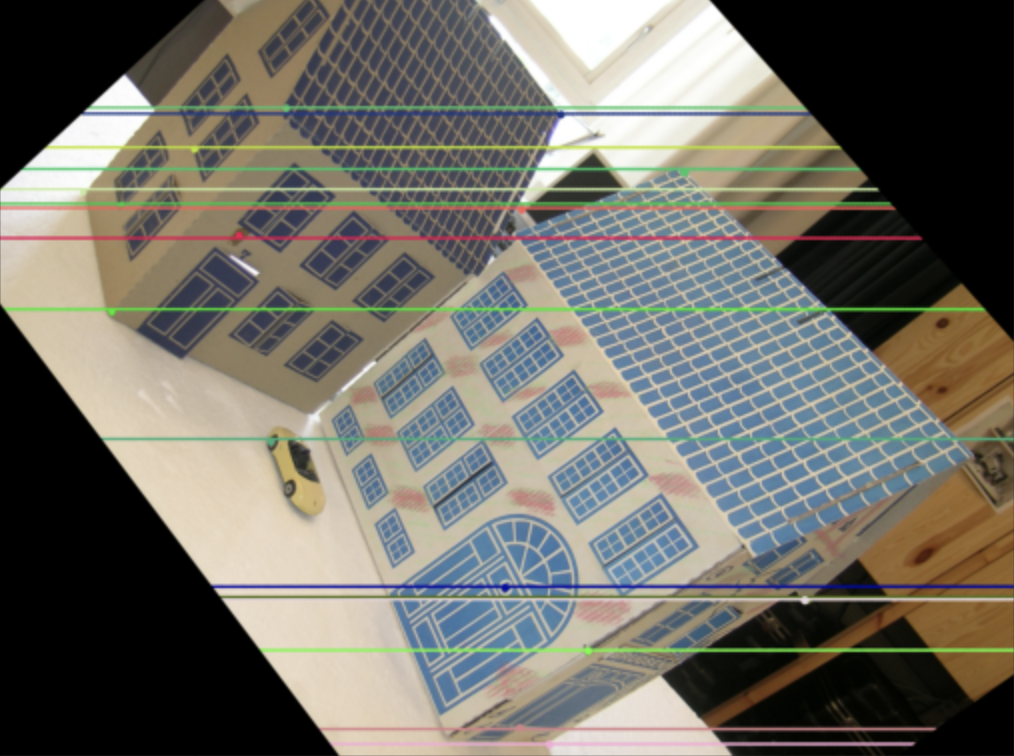
\includegraphics[width=\linewidth]{Materials/BaselineBRansac}
	\end{subfigure}
	\caption{Result of using Ransac on the original 25 correspondences before estimating the fundamental matrix and then bringing the images to scanline agreement.}
	\label{BaselineRansac}
\end{figure}
We here find a \textbf{mean} of \textbf{4.14} and a \textbf{standard deviation} of \textbf{2.57} of the scanline agreement error, which is a significant improvement over not using Ransac.
\subsection{Improved correspondences}
We will now improve our precision of our correspondences by applying the Harris corner detector. This has been done by extracting a small patch around our initial point location, and then run the Harris corner detector to find a more 'robust'/'easier to find again' location. Once these  points have then been found, we can estimate the fundamental matrix and scanline error to see if these improved points have an effect on the fundamental matrix estimation.

\subsubsection{Problems with Harris corner detection}
It is not obvious what the parameters for the Harris corner detector should be to give optimal results. Because a vast majority of the work in finding the improved points already was manual, I have tweaked the parameters for each original point until the Harris corner detector found a point which I would reckon would be easy to also find in the other image after applying the corner detector.\\
Another approach would have been to keep the parameters of the Harris corner detector constant and assume it is consistent. That is, if it does not find a perfect location, it will not find it in the other image either, but still find the same point in both image. In other words, if it makes a mistake, it make the same mistake in the other image. This would then have allowed us to discuss how well automatic detection could perform, whereas the first (and used) approach instead finds a 'lower bound' on the error we can get.

\subsubsection{Scanline agreement error}
If we simply estimate the fundamental with the improved correspondences we now find a \textbf{mean} of \textbf{1.92} and a \textbf{standard deviation} of \textbf{1.40} of the scanline agreement error. This is a fair bit better than running Ransac on the original correspondences, but as mentioned earlier, this is not representative for how an automatic detection would perform. We can now run Ransac on the improved correspondences and see the result in \autoref{ImprovedRansac}.

\begin{figure}[h]
	\centering
	\begin{subfigure}{0.48\linewidth}
		\centering
		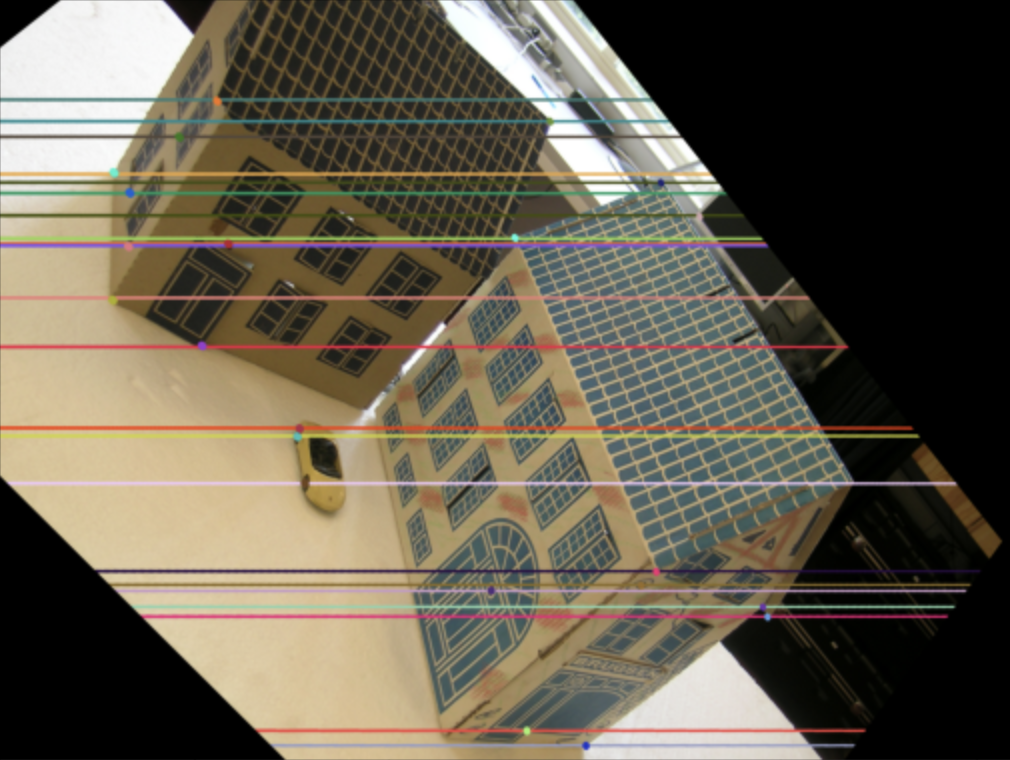
\includegraphics[width=\linewidth]{Materials/ImprovedARansac}
	\end{subfigure}
	\begin{subfigure}{0.48\linewidth}
		\centering
		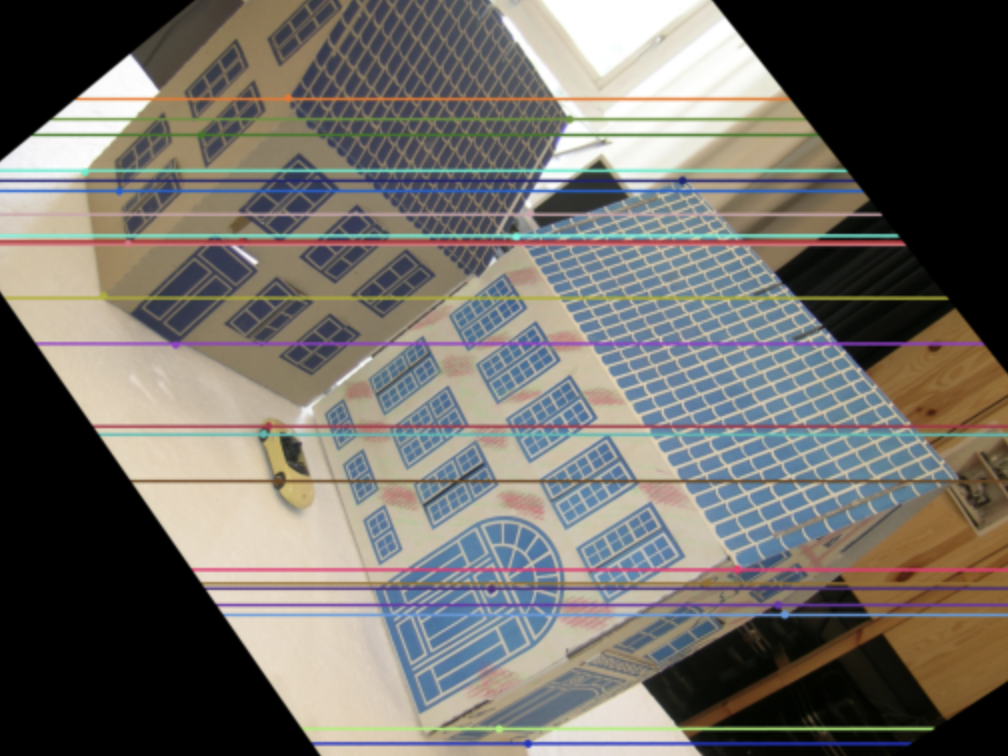
\includegraphics[width=\linewidth]{Materials/ImprovedBRansac}
	\end{subfigure}
	\caption{Result of using Ransac on the improved 25 correspondences before estimating the fundamental matrix and then bringing the images to scanline agreement.}
	\label{ImprovedRansac}
\end{figure}
We here find a \textbf{mean} of \textbf{1.52} and a \textbf{standard deviation} of \textbf{1.40} of the scanline agreement error, which is a slight improvement.

\subsubsection{Error as function of falsely added correspondences }
Looking at the error as a function of falsely added correspondences, now using the improved correspondences we get the results seen in \autoref{ImprovedRansacMedian}.

\begin{figure}[h]
	\centering
	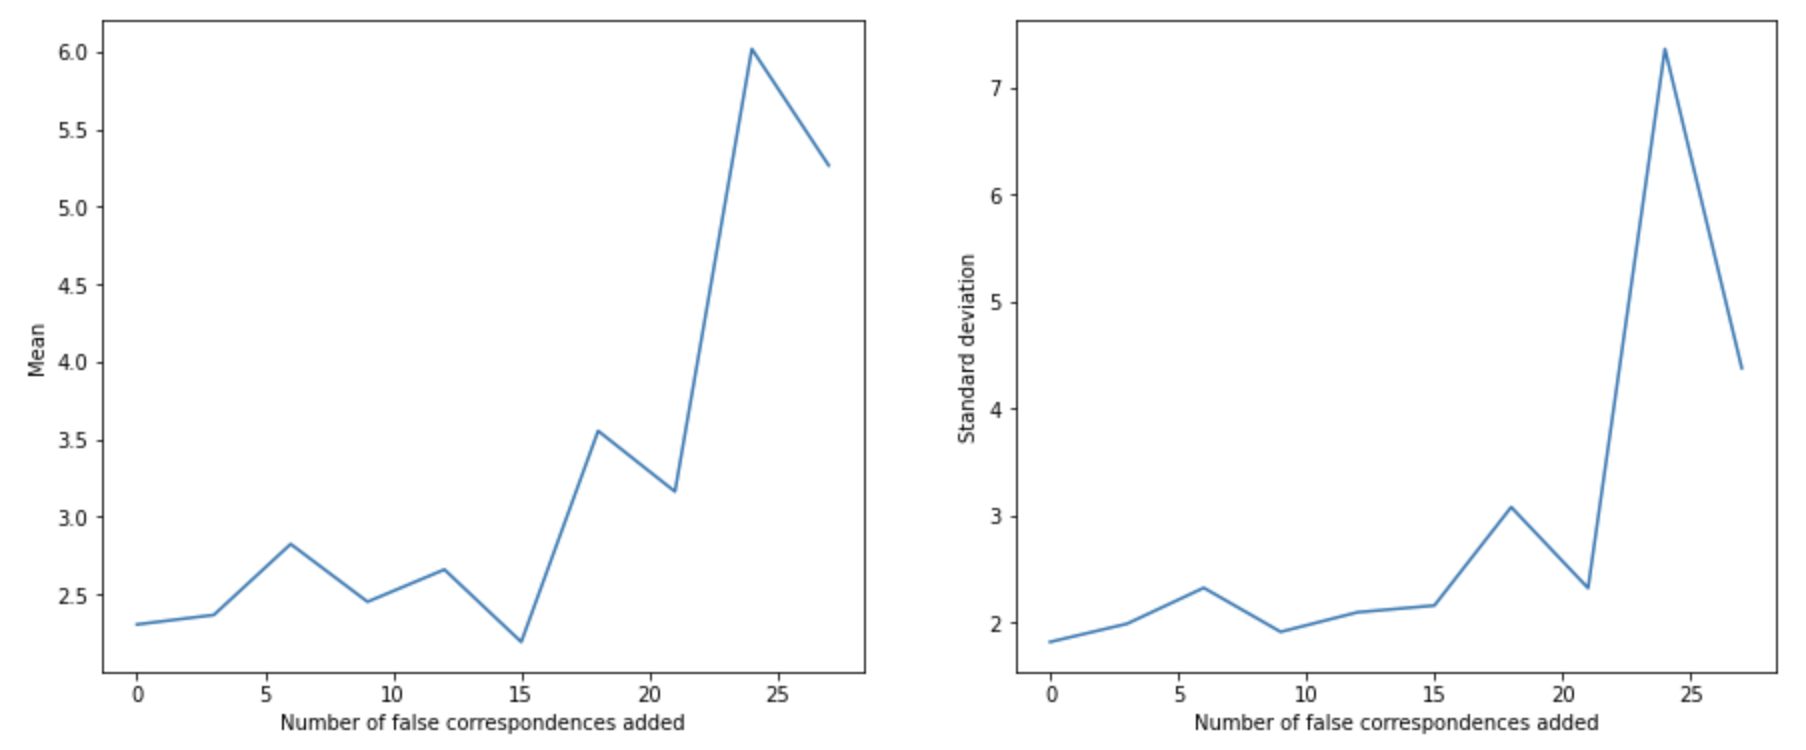
\includegraphics[width=\linewidth]{Materials/ImprovedRansacMedian}
	\caption{The median mean and standard deviation after 10 Ransac runs with increasing number of false correspondences added to the improved correspondences.}
	\label{ImprovedRansacMedian}
\end{figure}
We here see similar results as with the original correspondences, except a more clear tendency of increased error with increased number of false correspondences added. The more clear tendency might be a coincidence based on more similar Ransac runs or due to the run with 24 added false correspondences having a high error, and making it harder to see the small differences in mean and standard deviation. 
\subsection{Conclusion}
In conclusion we have seen SIFT and SURF detects roughly the same amount of features where ORB detects considerable less features. All three image descriptors perform somewhat bad when it comes to mean localization error, but this is likely due to aliasing or approximation error when transforming the images. When it comes to nearest neighbour mean average precision we see SIFT and ORB performs similar and fairly well, however SURF performs quite bad. This might be due to SIFT and ORB being both scale and rotation invariant, whereas SURF is only scale invariant. Lastly we have seen SIFT performs a lot better than both SURF and ORB when it comes to homography estimations, which is likely because SIFT both detects a lot of features and describes them well.\\
If we are to determine which of the three is better, it would depend on the task at hand. Although it is clear SIFT performs the best in the these experiments, it is also the slowest of the three. If the task requires fast feature matching it would not be possible to use SIFT, and we would need to trade performance for speed.
\section{Assignment 2}
Throughout this assignment we will use image A (\autoref{A}) and image B (\autoref{B}) to measure similarity. Both image have been downsampled and then blurred with a Gaussian kernel with sigma being 1. For the three similarity graphs, the results have been normalized such that all optima touch 1.0.
\begin{figure}[h]
	\centering
	\begin{subfigure}{0.4\linewidth}
		\centering
		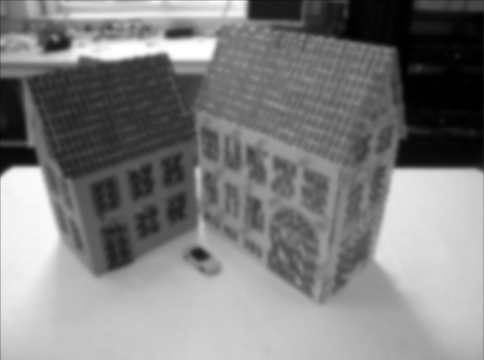
\includegraphics[width=\linewidth]{Materials/A}
		\caption{Image A.}
		\label{A}
	\end{subfigure}
	\hspace{1cm}
	\begin{subfigure}{0.4\linewidth}
		\centering
		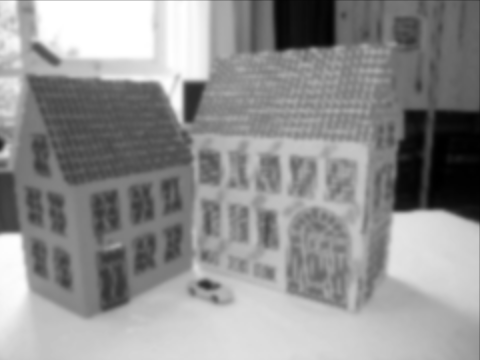
\includegraphics[width=\linewidth]{Materials/B}
		\caption{Image B.}
		\label{B}
	\end{subfigure}
	\caption{}
\end{figure}

\subsection{Self similarity}
We begin our examination of the four similarity measures by looking at self similarity. Here image A is compared to itself. The results can be seen in \autoref{self}.

\begin{figure}[h]
	\centering
	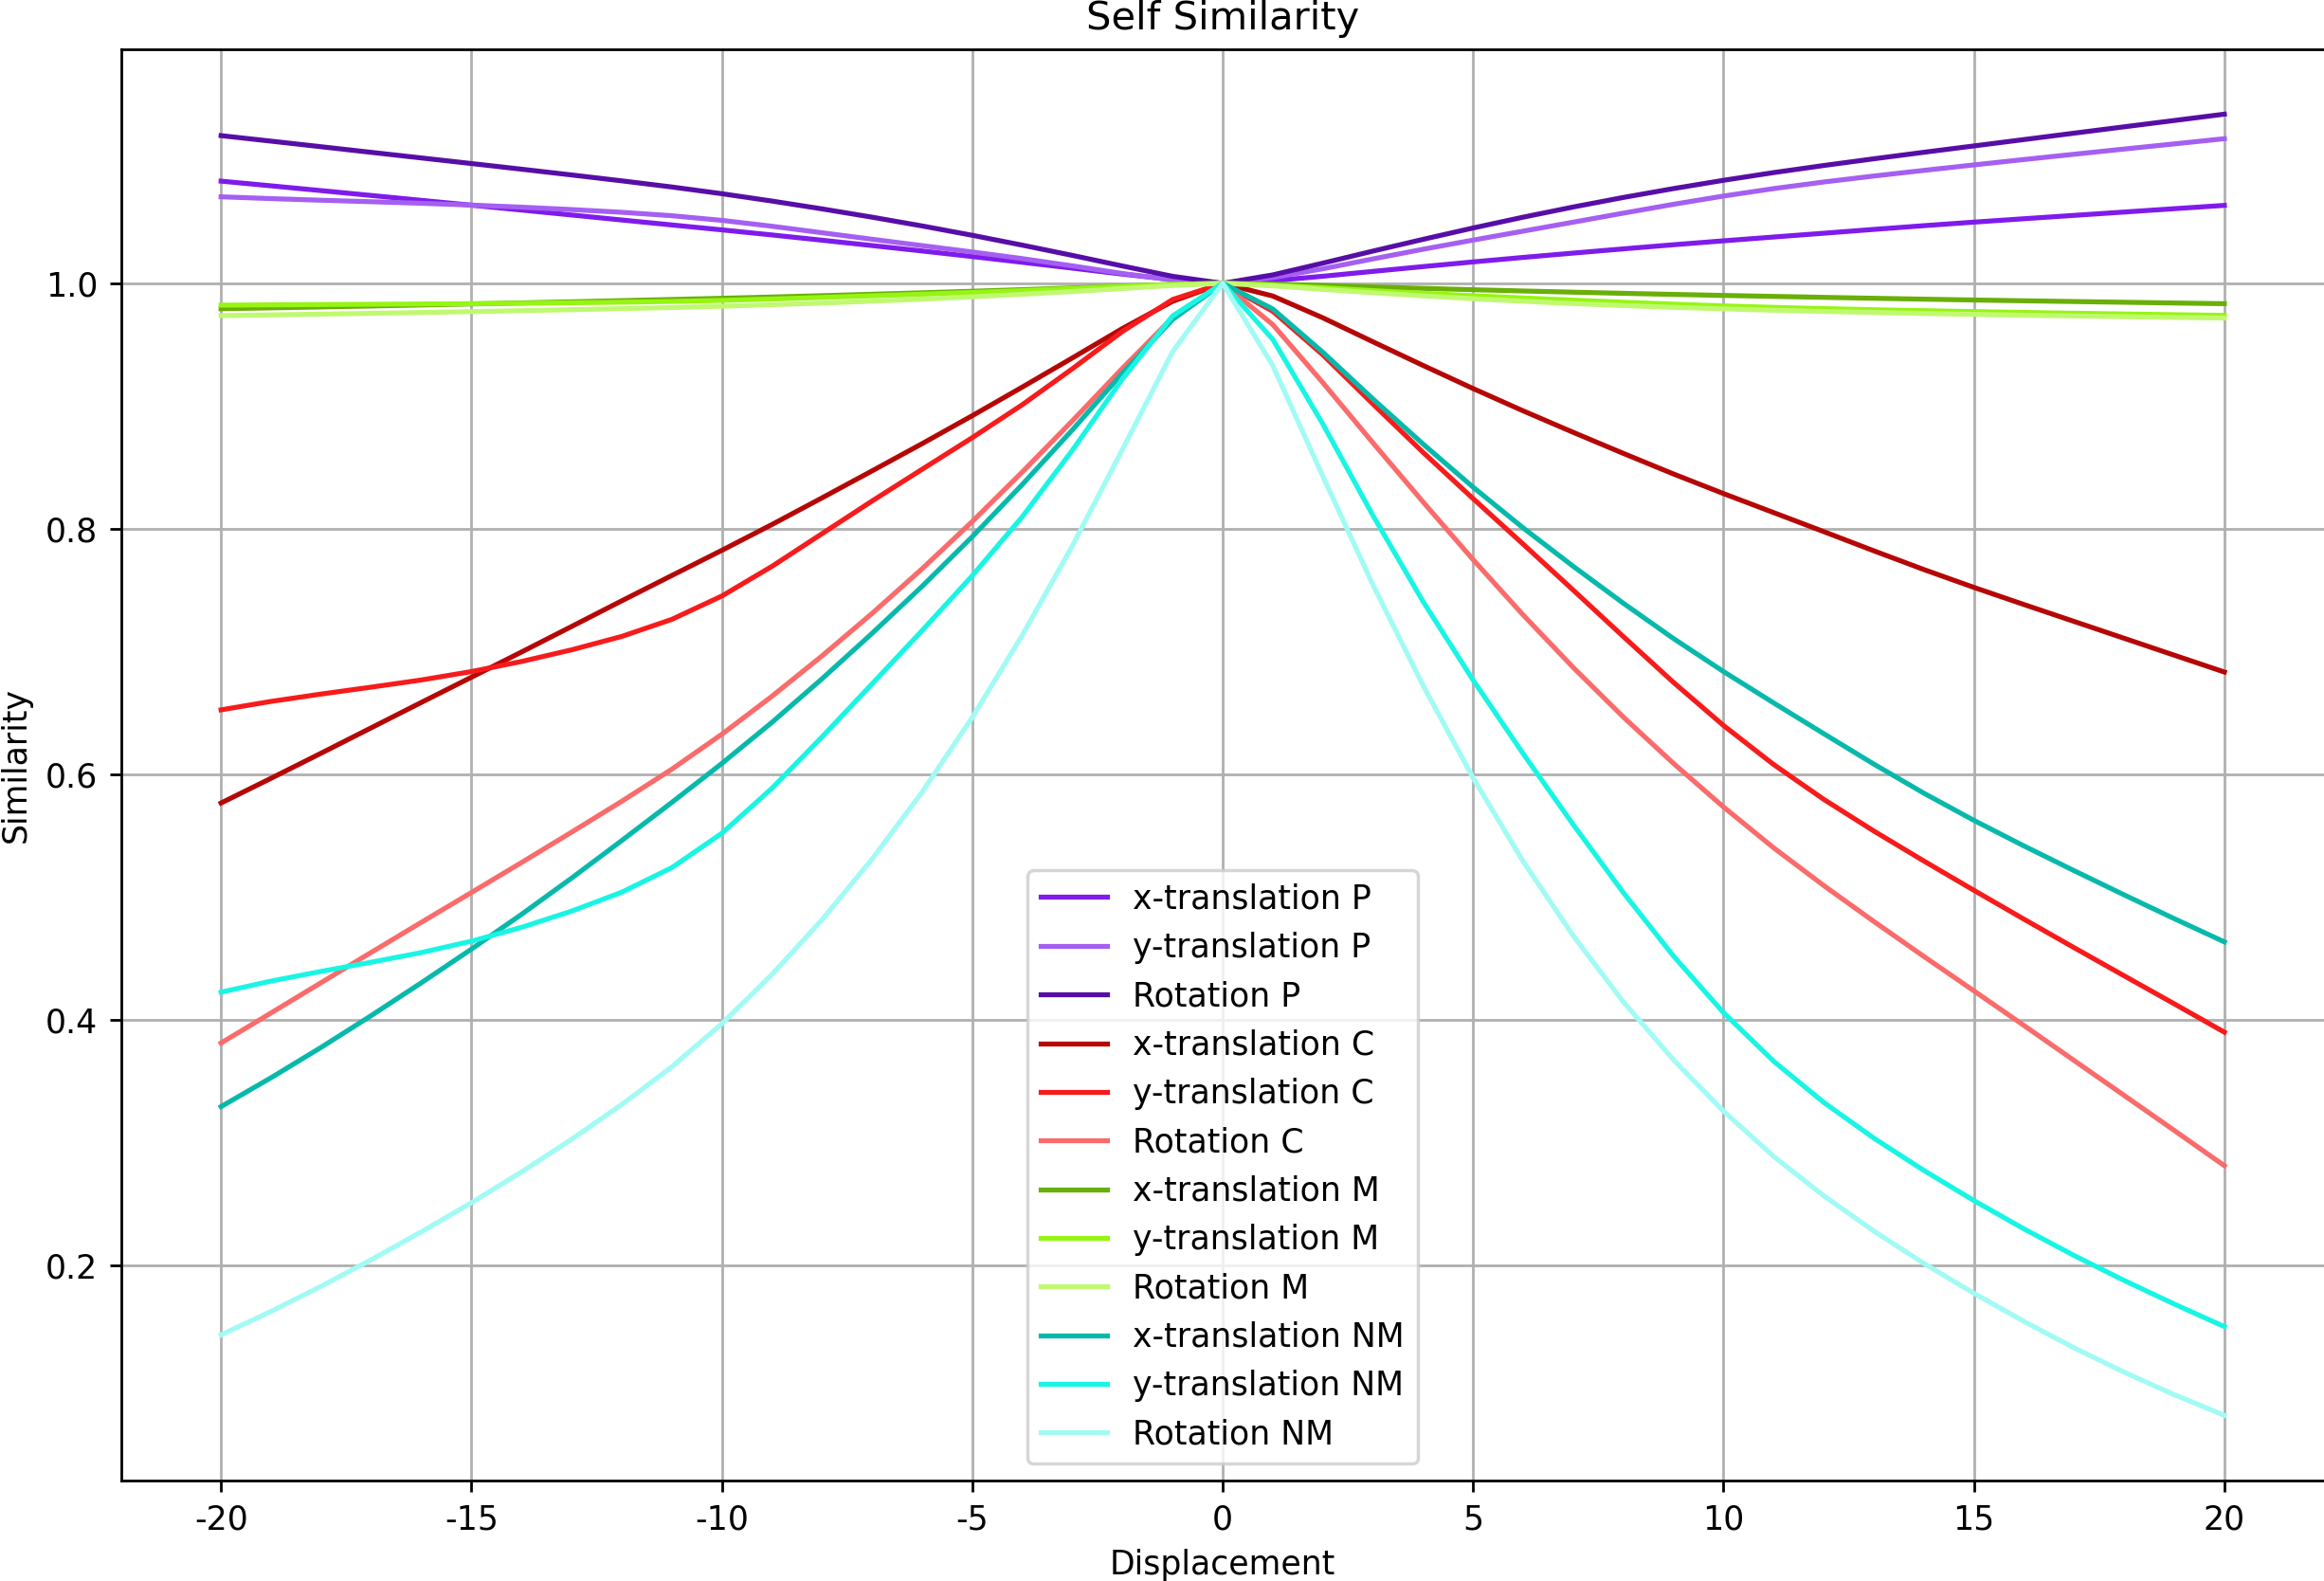
\includegraphics[width=0.8\linewidth]{Materials/selfSimilarity}
	\caption{Self similarity results normalized such that all optima touch 1.0. Both images have been blurred by a Gaussian kernel with sigma being 1. Translation displacement is measured in pixels and rotation displacement is measured in degrees. P = P-norm with P being 2, C = normalized cross correlation, M = mutual information, NM = normalized mutual information.}
	\label{self}
\end{figure}
From the results we note that all similarity measures should be maximized with the exception of P-norm, and thus the P-norm goes above 1.0. We can also see that the similarity measure with the biggest relative difference is NMI, which means NMI both have the greatest gradients, but also is the most sensitive to displacements. In comparison, we see that MI is almost completely flat. However, because MI is so flat, it makes the curves more smooth when we get close to 1.0, whereas for NMI we get some uneven sudden changes as we approach 1.0. For all similarity measures we see them 'peak' at 1.0 as expected as the images should be most similar when not displaced. 
\subsection{Multi modal similarity}
We now take a look at multimodal similarity. Here we have used image A and image A inverted, that is, the intensities have been multiplied by -1. The results can be seen in \autoref{multiModal}.

\begin{figure}
	\centering
	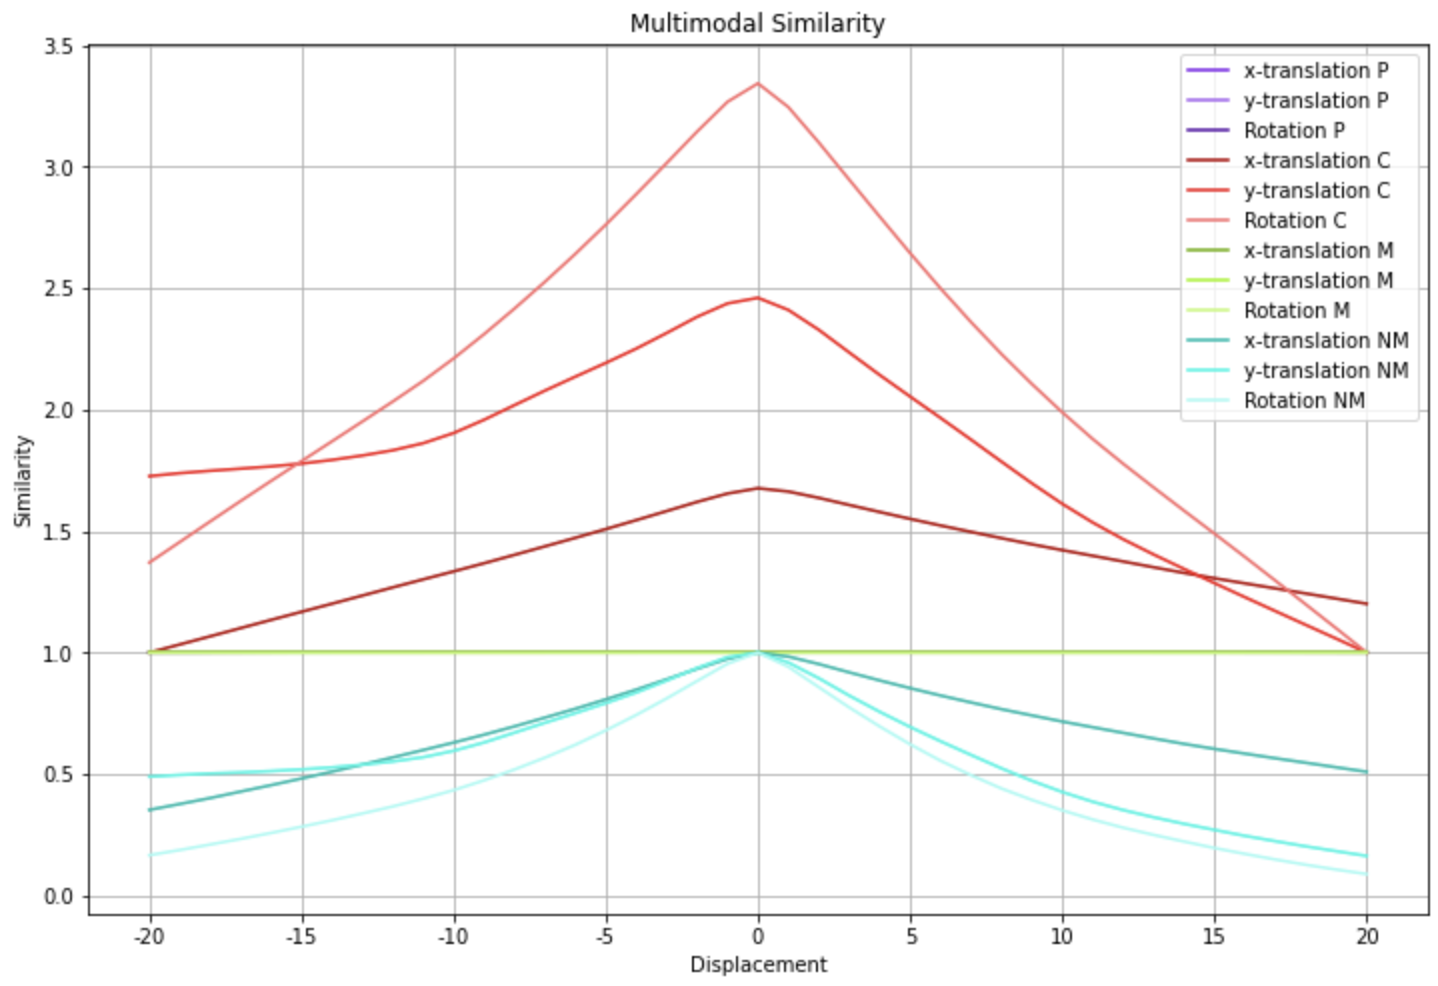
\includegraphics[width=0.8\linewidth]{Materials/multiModalSimilarity}
	\caption{Multi modal similarity results normalized such that all optima touch 1.0. Both images have been blurred by a Gaussian kernel with sigma being 1. Translation displacement is measured in pixels and rotation displacement is measured in degrees. P = P-norm with P being 2, C = normalized cross correlation, M = mutual information, NM = normalized mutual information.}
	\label{multiModal}
\end{figure}
Although it is hard to see, we have that the P-norm is slightly above 1.0 except when the displacements are greatest where it touches 1.0, and we have MI is slightly below 1.0 except when we have 0 displacement where it touches 1.0. We note that NCC now finds the optimal similarities when the displacements are greatest and the smallest similarity when the displacements are 0 as we have normalized the similarities such that the optima touches 1.0. This means NCC is not invariant to intensity changes, and thus is not suitable as a similarity measure for multi modal images. The same is the case for P-norm which also has its optima where the displacement is greatest. We see that  MI behaves correctly and thus is invariant to intensity changes, however, MI become extremely flat, and so its gradients are almost 0. This would make it very hard to optimize the similarity measure with a gradient based method, but it is smooth. Lastly we have NMI which also shows invariance to intensity changes and, of the correctly behaving similarity measures, shows the greatest sensitivity to the displacements. This makes the gradients bigger and thus the function easier to optimize. We also see the curves being more smooth than during self similarity.\\
The reason for P-norm and NCC not being invariant to these intensity changes is they both rely on intensities to compute the similarity, and thus, when we invert one of the images we get negative values as part of the similarity measures, which seemingly flips everything around the x-axis. As MI and NMI works on the distribution of the intensities, and not the intensities themselves, it does not matter if the values have been inverted, it only matter whether we observe as many inverted values as non-inverted values, i.e. that the distribution of pixels are the same in the two images.
\subsection{Object similarity}
We now look at the similarity between image A and B. The results can be seen in \autoref{object}.

\begin{figure}
	\centering
	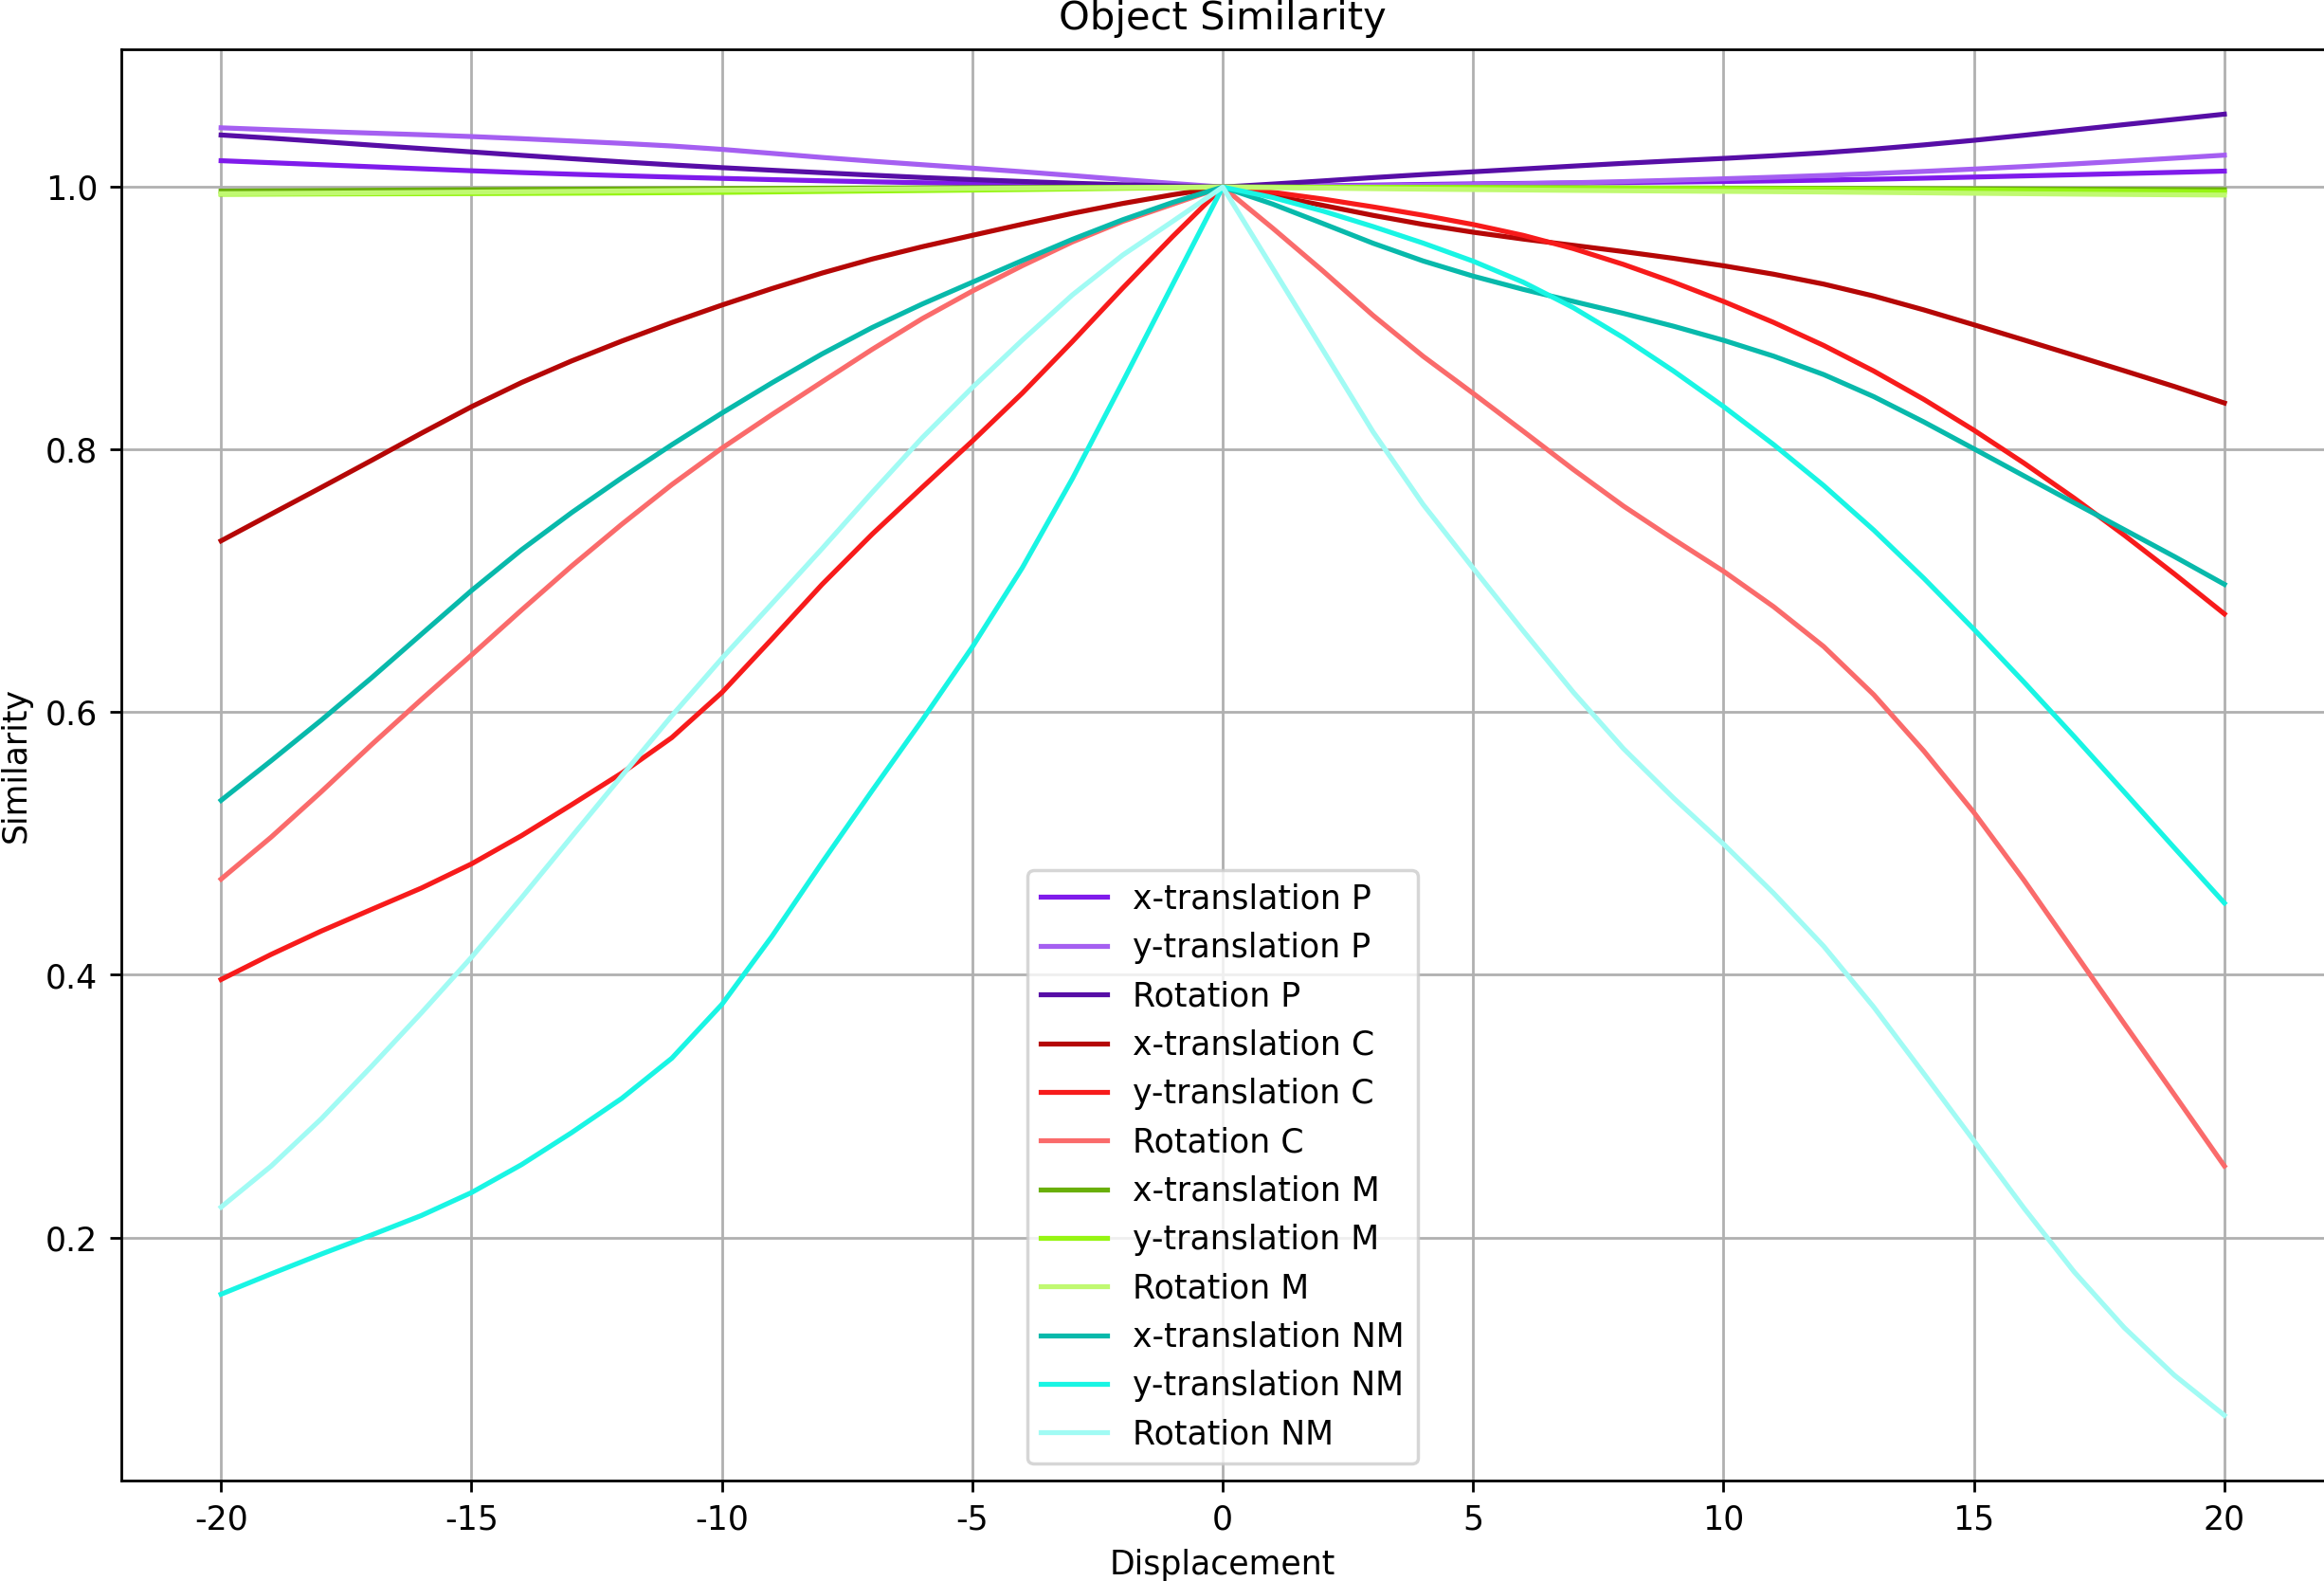
\includegraphics[width=0.8\linewidth]{Materials/objectSimilarity}
	\caption{Object similarity results normalized such that all optima touch 1.0. Both images have been blurred by a Gaussian kernel with sigma being 1. Translation displacement is measured in pixels and rotation displacement is measured in degrees. P = P-norm with P being 2, C = normalized cross correlation, M = mutual information, NM = normalized mutual information.}
	\label{object}
\end{figure}
We here see that all similarity measures again behaves correctly, however, compared to the self similarity results in \autopageref{self} the graphs have become more 'pointy' which would indicate the images are less similar as we need a smaller displacement to make the images dissimilar. By looking at the un-normalized similarity values it can also be reported that the similarity at optima has dropped for all similarity measure. However, we still see the optima being at 0 displacement. This might be due to the foreground and background being the most 'dominant' features in the images, and thus translating and rotating these out of the images might result in a bigger dissimilarity than aligning the images on the motif. We also see for NCC and NMI that the curves have become rather uneven / wavy and not as smooth as for self similarity. This is especially true around 1.0. The more wavy shapes of the curves could be an issue if we would like to optimize the functions with a gradient based method as the waves could form local minima and maxima. We see that the gradients of P-norm and MI is even more flat than for self similarity, making them hard to optimize. 
\subsection{Registration}
We can now look at how our similarity measures perform when we make a rigid and affine registration. In the simplest case we can make a rigid self registration (image A with image A) using NMI. Because we know an optimal transformation matrix will have $\theta = 0$, $t_x = 0$ and $t_y = 0$ we can initialize the transformation matrix to have $\theta = 0.2$, $t_x = 5$ and $t_y = 5$ and see if it returns to all zeros. If we let our gradient descend optimizer run for 200 iterations with a rotation learning rate of 1 and a translation learning rate of 100 we get that the final transformation matrix have $\theta =  0.0023$, $t_x = -0.039$ and $t_y = -0.014$ which is very close to our expectation.\\
We can now perform a rigid transformation using NMI again, but this time using image A and B. We begin by initializing $\theta = 0.3$, $t_x = 5$ and $t_y = 5$. The results can be seen in \autoref{rigidNMIAB}.

\begin{figure}[h]
	\centering
	\begin{subfigure}{0.4\linewidth}
		\centering
		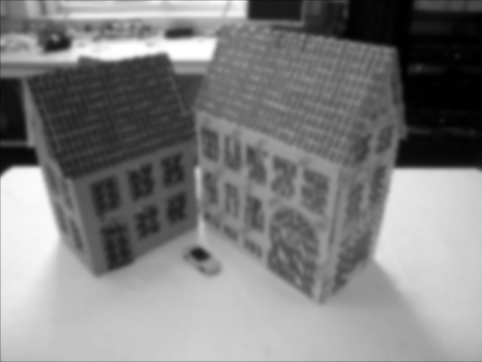
\includegraphics[width=\linewidth]{Materials/rigidNMIAB}
		\caption{Transformed image.\newline}
	\end{subfigure}
	\hspace{1cm}
	\begin{subfigure}{0.4\linewidth}
		\centering
		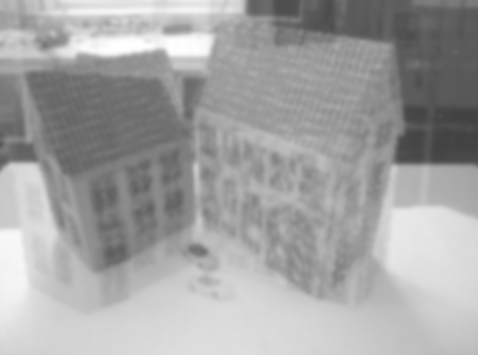
\includegraphics[width=\linewidth]{Materials/rigidNMIABO}
		\caption{Target image overlaid with transformed image.}
	\end{subfigure}
	\caption{Result of rigid registration using NMI on image A and B.}
	\label{rigidNMIAB}
\end{figure}
\begin{figure}
	\centering
	\begin{subfigure}{0.4\linewidth}
		\centering
		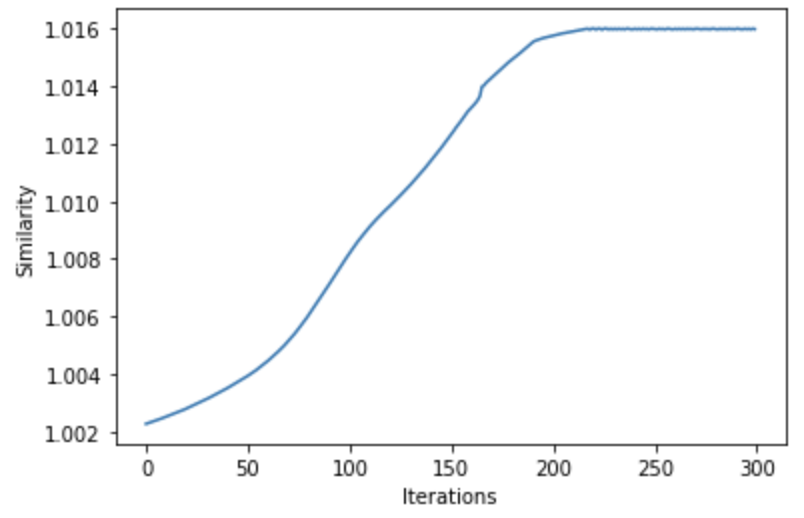
\includegraphics[width=\linewidth]{Materials/RigidNMILoss}
		\caption{Similarity using NMI at each iteration of optimization with translation learning rate of 100 and rotation learning rate at 1.}
		\label{rigidNMIABLoss}
	\end{subfigure}
	\hspace{1cm}
	\begin{subfigure}{0.4\linewidth}
		\centering
		\includegraphics[width=\linewidth]{Materials/RigidNCCLoss}
		\caption{Similarity using NCC at each iteration of optimization with translation learning rate of 10 and rotation learning rate at 0.1.}
		\label{rigidNCCABLoss}
	\end{subfigure}

\end{figure}
We see that the optimized transformation matrix goes towards 0 for all parameters which means it finds the optimal transformation to be no transformation. This is also consistent with the results seen in the object similarity section. In \autoref{rigidNMIABLoss} we see the similarity at each iteration of the optimization, and we see we have found an optima. As discussed earlier, the reason for the optimal parameters being 0 are probably because the foreground is dominant in the images, and optimizing the amount of foreground is probably better than optimizing the overlap of buildings.\\
We can now perform a rigid registration using NCC, image A and image B inverted. Here we initialize with the same parameters, but use a rotation learning rate of 0.1 and a translation learning rate of 10. The results can be seen in \autoref{rigidNCCAB}, and the similarity at each iteration can be seen in \autoref{rigidNCCABLoss}.

\begin{figure}[h]
	\centering
	\begin{subfigure}{0.4\linewidth}
		\centering
		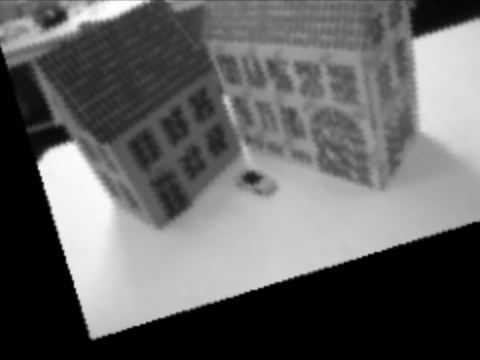
\includegraphics[width=\linewidth]{Materials/rigidNCCAB}
		\caption{Transformed image.\newline}
	\end{subfigure}
	\hspace{1cm}
	\begin{subfigure}{0.4\linewidth}
		\centering
		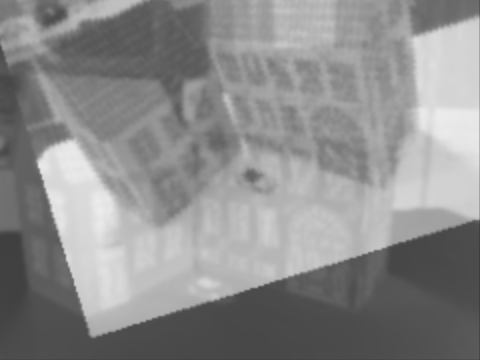
\includegraphics[width=\linewidth]{Materials/rigidNCCABO}
		\caption{Target image overlaid with transformed image.}
	\end{subfigure}
	\caption{Result of rigid registration using NCC on image A and inverted B.}
	\label{rigidNCCAB}
\end{figure}
We here note the motif is getting turned out of the resulting image. This is likely again because the foreground is attempted matched, and rotating the image introduces black pixels into the foreground. This illustrates that NCC is \textit{not} intensity invariant. We also note from \autoref{rigidNCCABLoss} that we have not yet reached an optima, which means if we ran more iterations or used bigger learning rates, the image would get further rotate.\\
We can now perform an affine registration using NMI and image A and B. We initialize the transformation matrix with the same $\theta$, $t_x$ and $t_y$ values as before and initialize $s_x = s_y = 1.2$. The rotation learning rate is set to 0.7, for translation it set to 100, and for scaling it is set to 1. The results can be seen in \autoref{affineNMIAB} and the similarity at each iteration can be seen in \autoref{affineNMIABLoss}.

\begin{figure}[h]
	\centering
	\begin{subfigure}{0.4\linewidth}
		\centering
		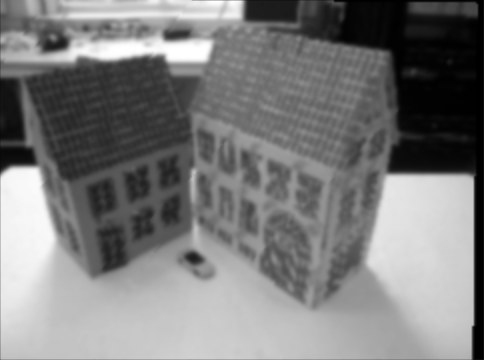
\includegraphics[width=\linewidth]{Materials/affineNMIAB}
		\caption{Transformed image.\newline}
	\end{subfigure}
	\hspace{1cm}
	\begin{subfigure}{0.4\linewidth}
		\centering
		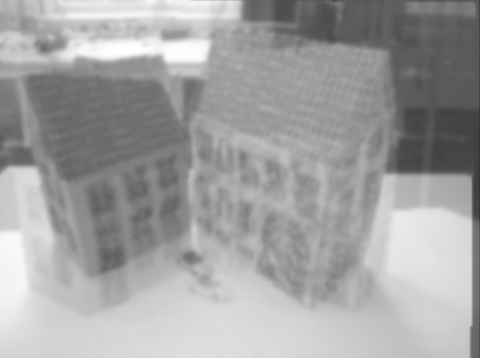
\includegraphics[width=\linewidth]{Materials/affineNMIABO}
		\caption{Target image overlaid with transformed image.}
	\end{subfigure}
	\caption{Result of affine registration using NMI on image A and B.}
	\label{affineNMIAB}
\end{figure}
\begin{figure}[h]
	\centering
	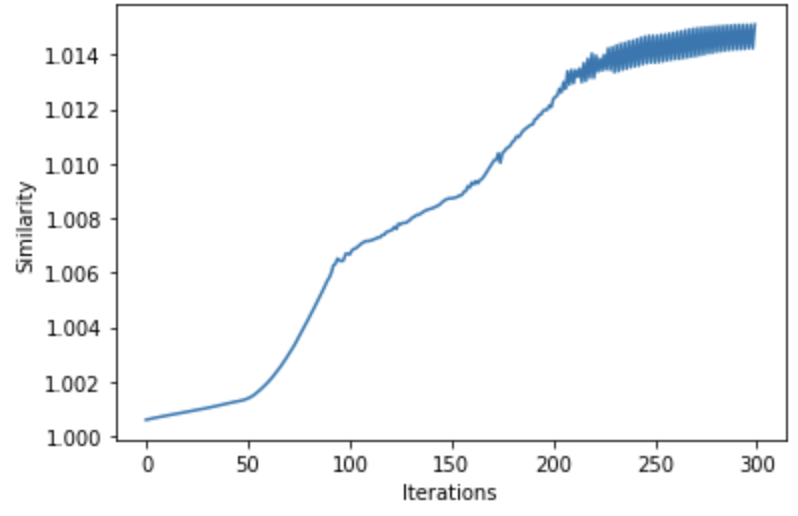
\includegraphics[width=0.4\linewidth]{Materials/affineNMIABLoss}
	\caption{Similarity at each iteration for affine registration between image A and B using NMI.}
	\label{affineNMIABLoss}
\end{figure}
We here note it is attempted to align the foreground of the images, however looking at \autoref{affineNMIABLoss} we see some volatile oscillation towards the end indicating we are using too big learning rates. This is likely the reason the the transformation matrix is not returning to 0 displacement. However, we see the houses and the car overlap slightly more than before. 
\subsection{Conclusion}
In conclusion we have seen SIFT and SURF detects roughly the same amount of features where ORB detects considerable less features. All three image descriptors perform somewhat bad when it comes to mean localization error, but this is likely due to aliasing or approximation error when transforming the images. When it comes to nearest neighbour mean average precision we see SIFT and ORB performs similar and fairly well, however SURF performs quite bad. This might be due to SIFT and ORB being both scale and rotation invariant, whereas SURF is only scale invariant. Lastly we have seen SIFT performs a lot better than both SURF and ORB when it comes to homography estimations, which is likely because SIFT both detects a lot of features and describes them well.\\
If we are to determine which of the three is better, it would depend on the task at hand. Although it is clear SIFT performs the best in the these experiments, it is also the slowest of the three. If the task requires fast feature matching it would not be possible to use SIFT, and we would need to trade performance for speed.
\section{Assignment 3}
\subsection{Design of experiments}
%When comparing images taken of the same scene, three common changes are scale, rotation and illumination. Because of this, I have designed my experiments to evaluate image descriptors on a roughly equal amount of images mainly varying in scale, rotation and illumination. 
For this assignment a subset of the 'HPatches' data set has been chosen, namely the first 10 series with illumination changes and the 10 fist series with view point changes. Three image descriptors, namely SIFT, ORB and SURF will then be evaluated on the aforementioned data. A consideration for the experiments have been, that an image descriptor both chooses a location in an image which it finds fitting, and it describes this location. That is, we both get key points and descriptors for each found feature in the image. To evaluate the key points we use \textit{mean localization error}, to evaluate descriptors we use \textit{nearest neighbour mean average precision}, and to evaluate the image descriptor as a whole, we use \textit{homography estimation}. Before going into details with these error measures, we will first look at how we classify true positives, false positives and false negative detections.\\
For each pair of images considered, we apply the image descriptor to both images, and the detections made in \textit{image 1} are considered ground truth whereas the detections made in \textit{image 2} are considered candidate points. If there is a perspective change between the two images, the ground truths are warped into the perspective of the candidate points. To detect false positives, we go through each detection in our candidate points, and each candidate point which does not have a similar ground truth is considered a false positive. To detect false negatives we go through each ground truth and if it does not have a similar candidate point it is a false negative. A true positive can be measured as either each candidate point which has a similar ground truth, or each ground truth which has a similar candidate point. This 'similar' / $\epsilon$ term is measured as the L2 norm, and can be increased / shrunk in order to create precision / recall curves. We will compute precision and recall by starting with $\epsilon = 0$ and increase it.
As we might have more ground truths than candidate points and vice versa, the recall and precision is rescaled to always go from 0 to 1. 
To ensure correct curves, 1 - recall will be used to compute precision / recall curves. An example of a precision / recall curve can be seen in \autoref{PRCurve}. Each ground truth or candidate point can only be matched once, that is, if we have two candidate points around a ground truth, only one of them will be considered a true positive whereas the other will be considered a false positive.\\
\textit{opencv} implementations of the image descriptors have been used, and all image descriptors have their default parameters.

\begin{figure}[h]
	\centering
	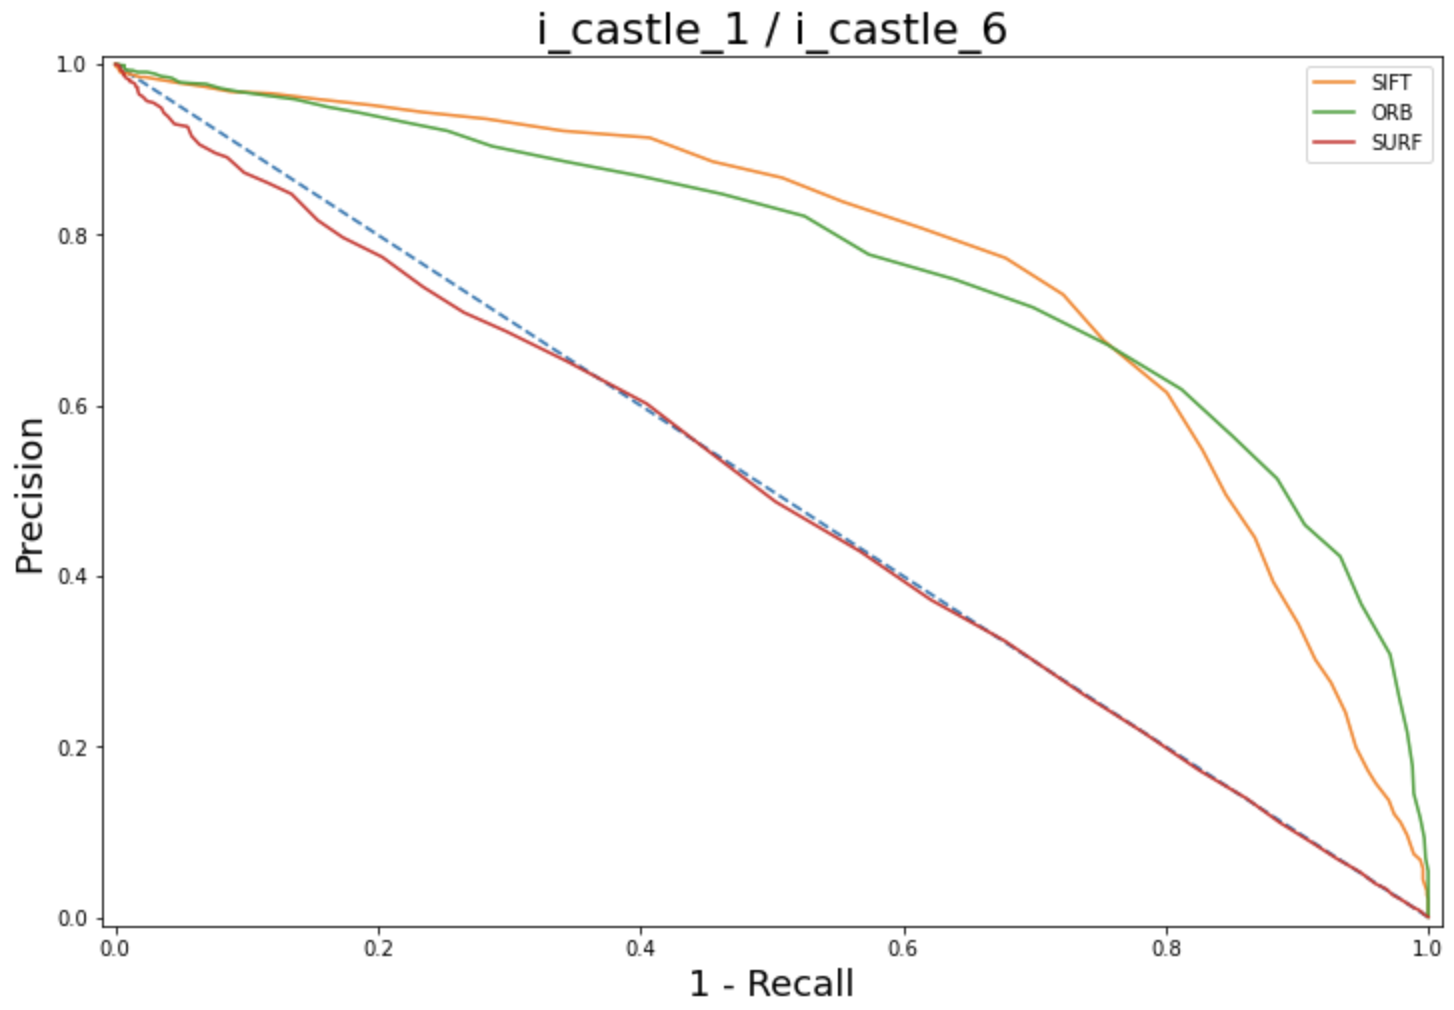
\includegraphics[width=0.68\linewidth]{Materials/PRCurve}
	\caption{Precision / recall curve for two images in the castle series.}
	\label{PRCurve}
\end{figure}
\subsection{Error measures}
We can now discuss the definition of each error measure.\\
\textit{Mean localization error} is defined in accordance to \cite{sp} where we only use true positive detections and find the average distance between their nearest neighbours. This measure tells us about how close the key points are to each other in the two images, that is, if the image descriptor finds the same points in the two images. The error ranges between 0 and $\epsilon$, where $\epsilon$ is the maximum distance between the two key points there can be for them to be considered true positives. As it is unclear which epsilon is used in \cite{sp}, I have chosen to report the mean localization error for a range of epsilon values. To avoid rewarding image descriptors which find 0 features, the maximum error ($\epsilon$) is used for a run where 0 features are found.\\
\textit{Nearest neighbour mean average precision} is defined in accordance to \cite{sp}, and takes all descriptors of an image pair and finds their nearest neighbour. Then creates a precision / recall curve and measures the area under the curve for this image pair. Then the average area under the curve is estimated across all image pairs. This measure estimates how well the image descriptor detects true positives without introducing false positives. The measure ranges between 0 and 1. As we are comparing the same scene, the descriptions made should describe the same image patches, and thus we do not perform any perspective warping for this measure. As it is not clear from \cite{sp} which range of $\epsilon$ values are used, I have chosen to use 100 evenly spaced $\epsilon$ values between 100 - 800 as the distance between all found descriptors in the manually inspected images seem to be matched in this range. To make this measure computational feasible, only the first 1000 descriptors found are used. These are likely in the same part of the image, but sampling 1000 descriptors across the image might result in a lot of descriptors which are not measured at the same key points.\\
\textit{Homography estimation} is defined in accordance to \cite{sp} and takes the four corners of \textit{image 1} and first measures the average distance between each corresponding corner transformed by the true homography matrix and the estimated homography matrix found by taking nearest neighbour matches found by the image descriptor. If the average distance is less than some $\epsilon$ then it is reported as a correct homography estimation, otherwise it is reported as a wrong estimation. The average number of correct estimations over all image pairs is then reported as the \textit{homography estimation} measure. This measure evaluates the image descriptor as a whole by taking points matched in the two images to estimate a homography to warp one image into the perspective of the other. The result ranges between 0 and 1. As SIFT returns \textit{a lot} of features, a Lowe's ratio at $0.7$ is used to filter the number of features used to estimate the homography.
\subsection{Results}
To get an idea of how many features each image descriptor produces, we will begin this section by taking a look at three image pairs where each image descriptor have been run. The found features can be seen in \autoref{noFeatures}, and only shows correct correspondences. By manual inspection, it can also be reported that in general (when not constrained) SIFT and SURF produces more matches than ORB.

\begin{figure}[h]
	\centering
	\begin{subfigure}{0.8\linewidth}
		\centering
		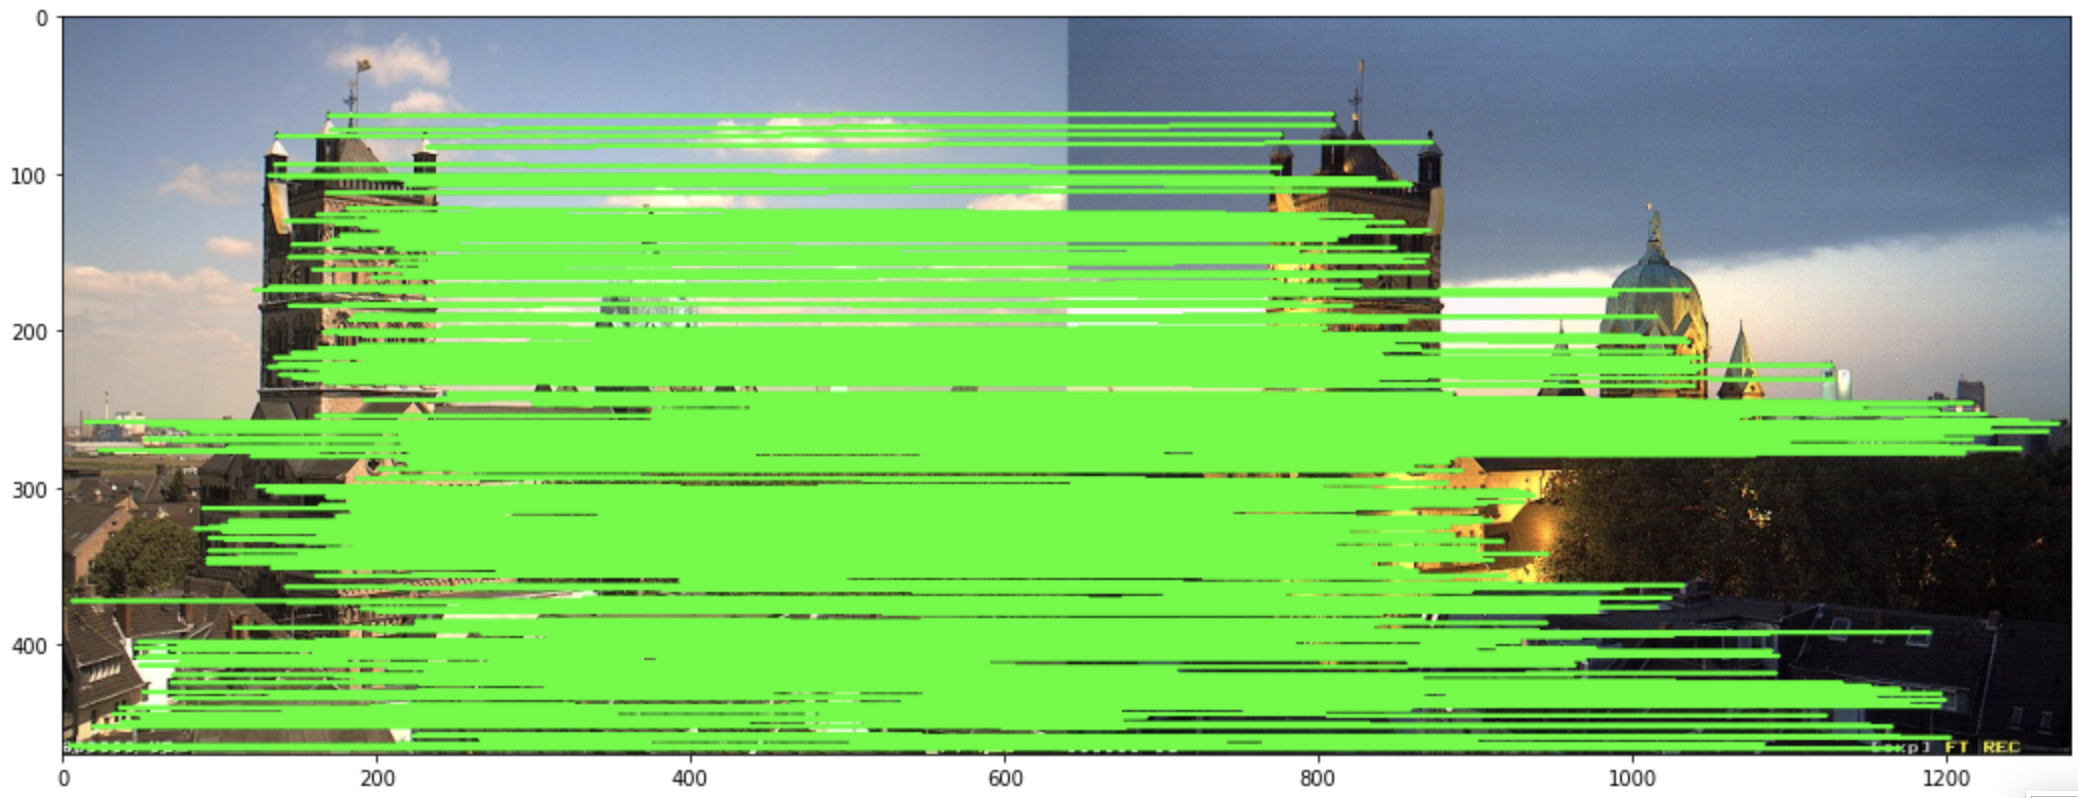
\includegraphics[width=\linewidth]{Materials/SIFTMatches}
		\caption{The detected SIFT features.}
	\end{subfigure}
	\\
	\begin{subfigure}{0.8\linewidth}
		\centering
		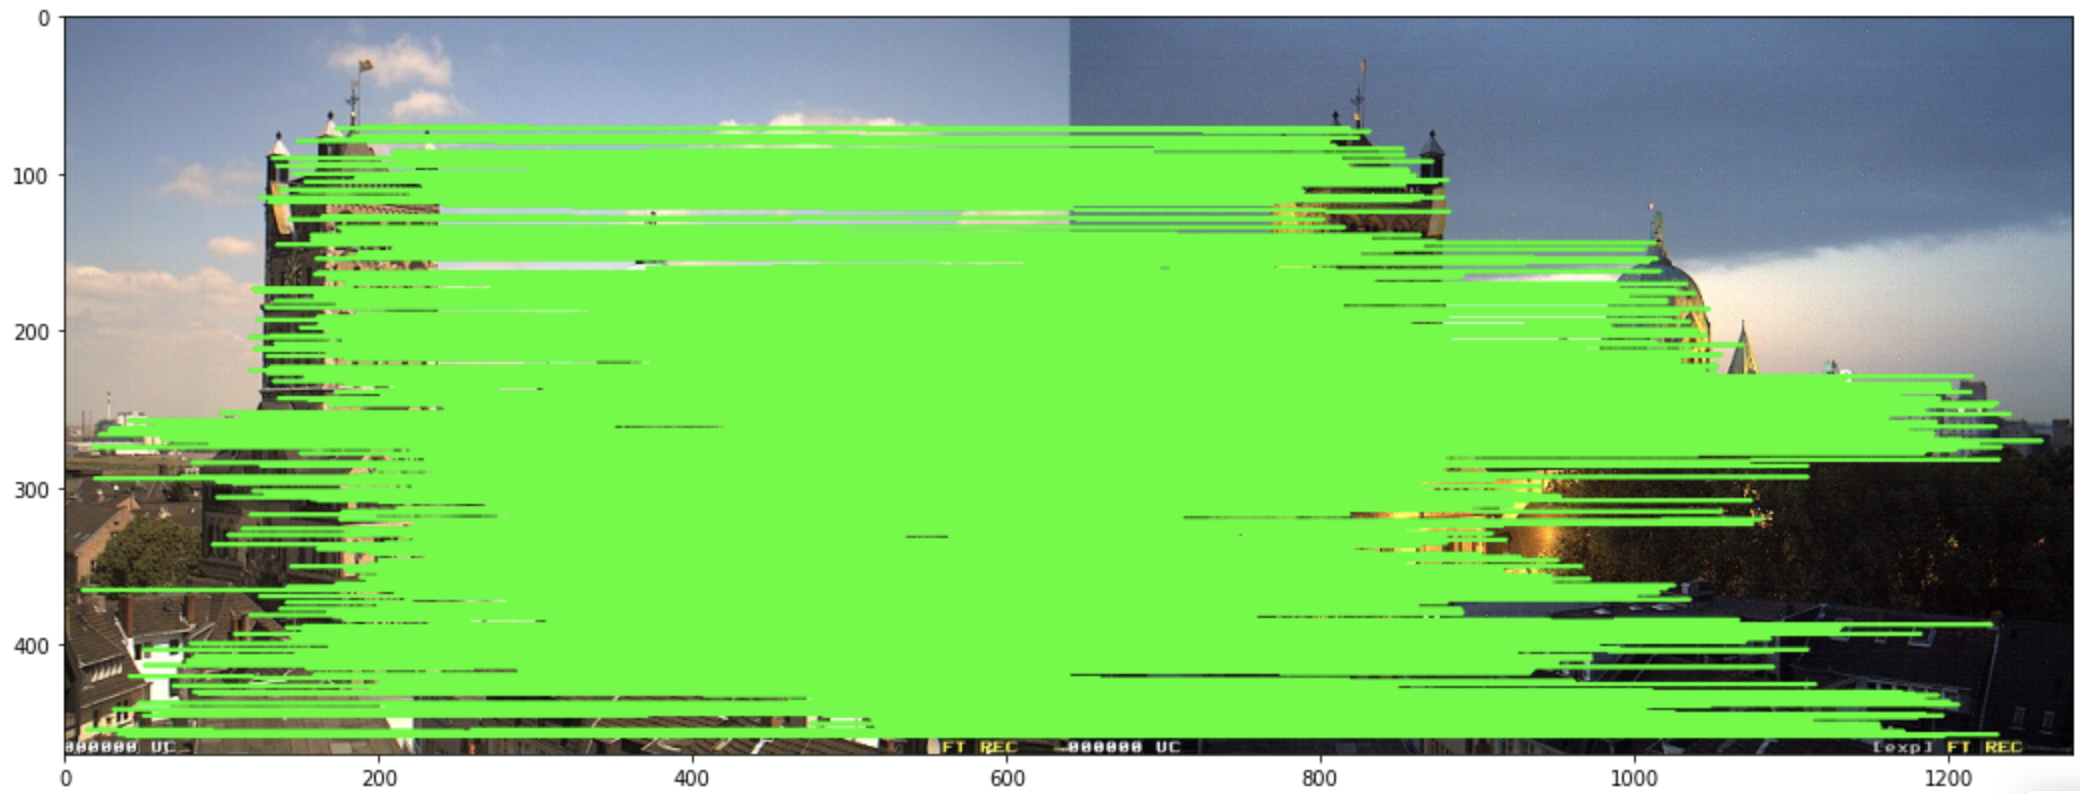
\includegraphics[width=\linewidth]{Materials/SURFMatches}
		\caption{The detected SURF features.}
	\end{subfigure}
	\\
	\begin{subfigure}{0.8\linewidth}
		\centering
		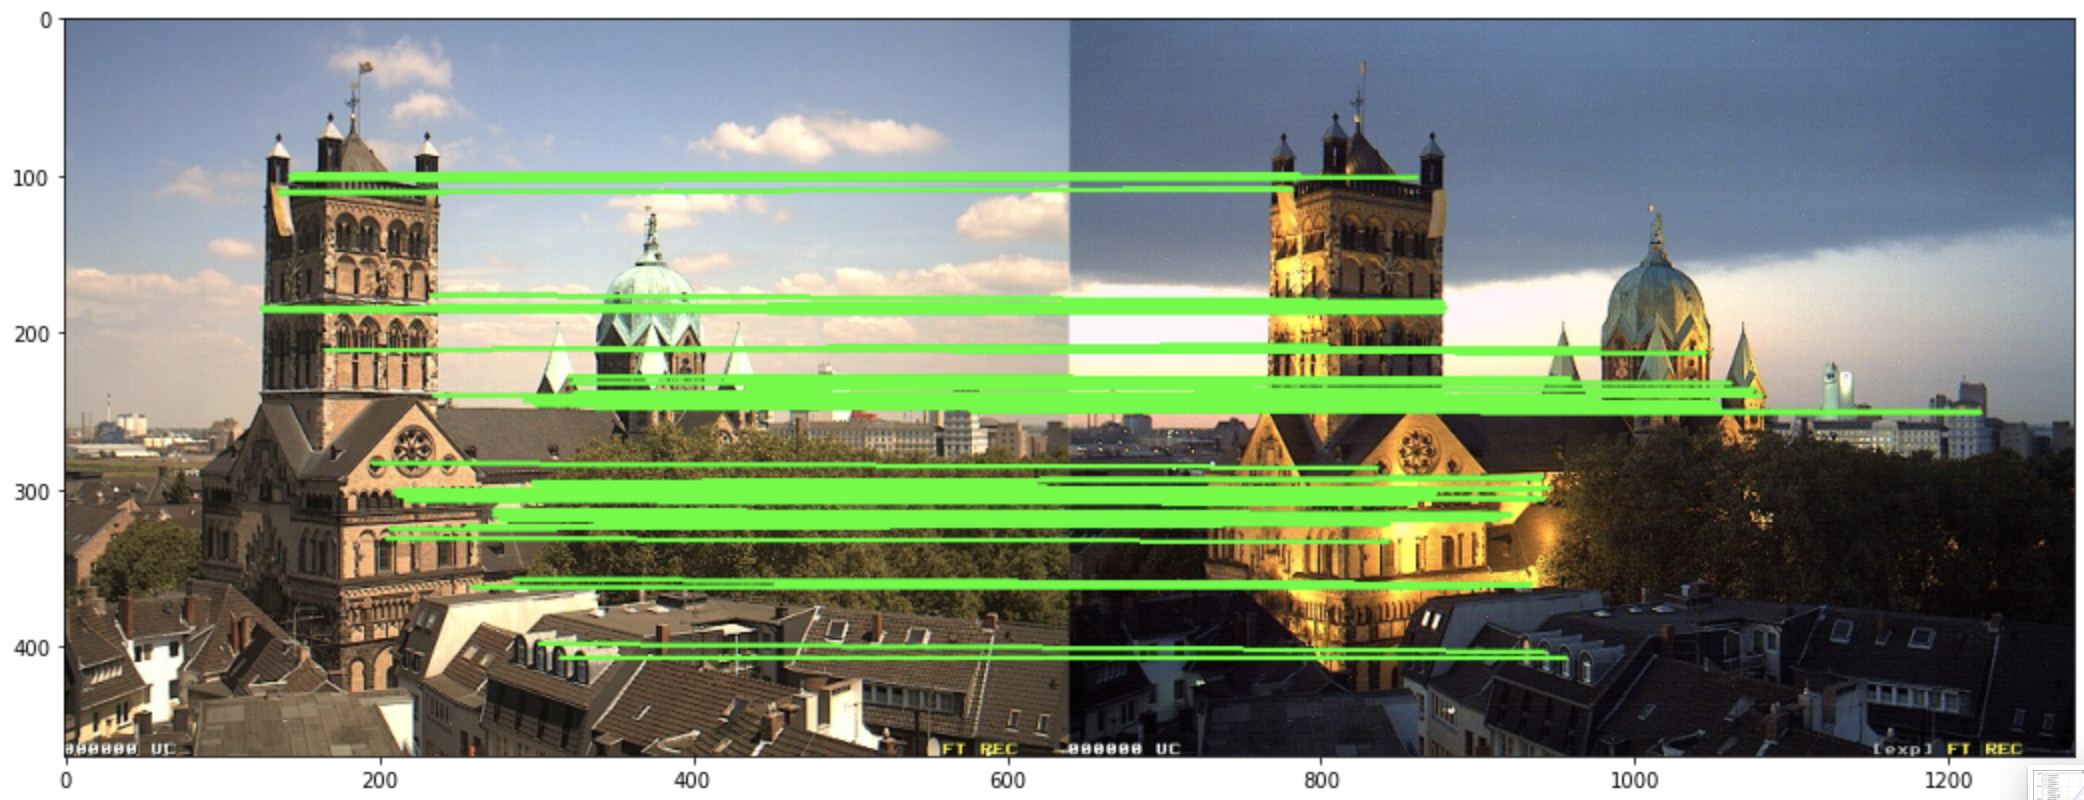
\includegraphics[width=\linewidth]{Materials/ORBMatches}
		\caption{The detected ORB features.}
	\end{subfigure}
	\caption{Each image descriptor run on the same image pair to give an indication of how many features each finds.}
	\label{noFeatures}
\end{figure}

\begin{table}[h]
	\centering
	\begin{tabular}{|c||ccc||ccc||c|}
		\hline
		& \multicolumn{3}{c||}{Homography estimation}                           & \multicolumn{3}{c||}{Mean localization error}                          & NN mean average precision \\ \hline
		& \multicolumn{1}{c|}{eps = 1} & \multicolumn{1}{c|}{eps = 3} & eps = 5 & \multicolumn{1}{c|}{eps = 1} & \multicolumn{1}{c|}{eps = 3} & eps = 5 &                           \\ \hline
		SIFT & \multicolumn{1}{c|}{0.34}   & \multicolumn{1}{c|}{0.61}    & 0.71    & \multicolumn{1}{c|}{0.56}    & \multicolumn{1}{c|}{1.46}    & 2.41    & 0.72                      \\ \hline
		ORB  & \multicolumn{1}{c|}{0.05}   & \multicolumn{1}{c|}{0.21}    & 0.31    & \multicolumn{1}{c|}{0.54}    & \multicolumn{1}{c|}{1.54}    & 2.41    & 0.73                      \\ \hline
		SURF & \multicolumn{1}{c|}{0.29}   & \multicolumn{1}{c|}{0.53}    & 0.66    & \multicolumn{1}{c|}{0.56}    & \multicolumn{1}{c|}{1.48}    & 2.27    & 0.50                      \\ \hline
	\end{tabular}
	\caption{Results of the experiments.}
	\label{results}
\end{table}
As seen, SIFT finds about as many features as SURF whereas ORB finds a considerable amount less.\\
In \autoref{results} we see the results of the experiments conducted. When comparing SIFT and ORB we see their ability to estimate correct homographies varies greatly. ORB estimates as many correctly homographies when epsilon is 5 as SIFT does when epsilon is 1, that is, SIFT is much more accurate when estimating homographies. SURF lies in between the two, performing closer to SIFT than ORB. However, when we compare the mean localization error SIFT, SURF and ORB obtain similar errors. This means their ability to choose the same places in the image pairs are equivalent. However, looking at the actual errors, we see the error is about halfway between the minimum and maximum possible which means we are fairly far away from the actual location we were looking for. When it comes to nearest neighbour mean average precision SIFT and ORB performs similar and fairly well, whereas SURF performs quite poorly.
\subsection{Discussion of results}
A reason for the big difference in homography estimation performance between SIFT and ORB might be how many feature points each find and are able to match. SIFT does find a considerable amount more features than ORB does, and because SIFT have more points, and point matches, it is able to estimate the homography better. RANSAC is used to eliminate outliers, which means even though SIFT might find more false positive matches, some are eliminated. It is likely SURF performs better than ORB for the same reason, however, because SURF produces worse descriptors (seen from nearest neighbour mean average precision) than SIFT, it is worse at estimating the homographies than SIFT.\\
The fact the mean localization error seems to be fairly high for all image descriptors might be due some aliasing or other approximation of the new location after moving the ground truth point locations into the coordinate system of the candidate points. If the new point location is off by 1 or 2 pixels it will make a quite big error in the mean localization error.\\
We see ORB and SIFT performs fairly well on nearest neighbour mean average precision, which is likely because they both are scale and rotation invariant, however, SURF is not rotation invariant, and this might be the reason it performs a lot worse. Another consideration when comparing nearest neighbour mean average precision is the length the descriptor vectors. SIFT creates a vector with length 128, ORB's descriptor vector length is 32 and SURF produces descriptors with length 64. When we measure the distance between these vectors the higher dimensional vectors are more likely to lie far away from each other. Having this in mind, SIFT seems to describe its features more accurately than ORB although their score is about the same.

\subsection{Conclusion}
In conclusion we have seen SIFT and SURF detects roughly the same amount of features where ORB detects considerable less features. All three image descriptors perform somewhat bad when it comes to mean localization error, but this is likely due to aliasing or approximation error when transforming the images. When it comes to nearest neighbour mean average precision we see SIFT and ORB performs similar and fairly well, however SURF performs quite bad. This might be due to SIFT and ORB being both scale and rotation invariant, whereas SURF is only scale invariant. Lastly we have seen SIFT performs a lot better than both SURF and ORB when it comes to homography estimations, which is likely because SIFT both detects a lot of features and describes them well.\\
If we are to determine which of the three is better, it would depend on the task at hand. Although it is clear SIFT performs the best in the these experiments, it is also the slowest of the three. If the task requires fast feature matching it would not be possible to use SIFT, and we would need to trade performance for speed.

\begin{thebibliography}{9}
	\bibitem{rectificationError}
	Monnase, P., et. al. 'Three-step image rectification'.  British Machine Vision Conference.  Aug 2010.
	
	\bibitem{sp}
	DeTone, D., et. al. 'SuperPoint Self-Supervised Interest Point Detection and Description'.  Unknown publisher.  Apr 2018.
\end{thebibliography}

\section{Collaboration}
Throughout the course I have been collaborating with Marcus Hansen on both code and discussion of course content.

\end{document}